\setcounter{section}{2}
\section{ĐA GIÁC ĐỀU VÀ PHÉP QUAY} % Tên bài
\subsection{Kiến thức trọng tâm}
\subsubsection{Đa giác đều}
\begin{tomtat}
	\begin{itemize}
		\immini{\item \textit{Đa giác} $ABCDE$ là hình gồm các đoạn thẳng $AB$, $BC$, $CD$, $DE$ và $EA$, trong đó bất kì hai đoạn thẳng nào có một điểm chung cũng không cùng nằm trên một đường thẳng.\\
		 Đa giác $ABCDE$ có năm đỉnh là các điểm $A$, $B$, $C$, $D$, $E$; năm cạnh là $AB$, $BC$, $CD$, $DE$, $EA$ và năm góc là $\widehat{ABC}$, $\widehat{BCD}$, $\widehat{CDE}$, $\widehat{DEA}$, $\widehat{EAB}$.}
		{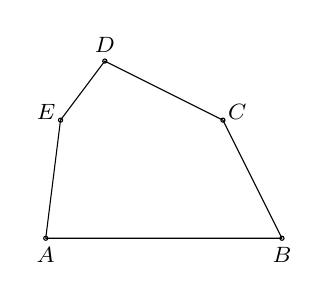
\begin{tikzpicture}[>=stealth,line join=round,line cap=round,font=\footnotesize,scale=.75]	
		\path (0,0)coordinate (A)
		(4,0)coordinate (B)
		(3,2)coordinate (C)
		(1,3)coordinate (D)
		(.25,2)coordinate (E);		
		\draw (A)--(B)--(C)--(D)--(E)--cycle;
		\foreach \x/\i in {A/-90,B/-90,C/30,D/90,E/150}{
			\draw(\x)circle (1pt)+(\i:8pt)node{$\x$};
			}
		\end{tikzpicture}
	}
		\item \textit{Đa giác lồi:} Nếu với một cạnh bất kì, các đỉnh không thuộc cạnh đó đều nằm về một phía đối với đường thẳng chứa cạnh đó thì đa giác được gọi là đa giác lồi.
		\item \textit{Đa giác đều:} Đa giác đều là một đa giác lồi có các cạnh bằng nhau và các góc bằng nhau.
	\end{itemize}
	Các hình dưới đây là hình các đa giác đều thường gặp.
	\begin{center}
		\begin{tikzpicture}[>=stealth,line join=round,line cap=round,font=\footnotesize,scale=1.2]	
			\node at (0,-1) {Hình tam giác đều};
			\node at (3,-1) {Hình vuông};
			\node at (6,-1) {Hình ngũ giác đều};
			\node at (9,-1) {Hình lục giác đều};
			%Hình tam giác đều
			\path (0,0) coordinate (O1)++(90:1) coordinate (A)	
			(O1)++(-30:1) coordinate (B)
			(O1)++(-150:1) coordinate (C);
			\draw (A)--(C)--(B)--(A);
			%Hình vuông
			\path (3,0) coordinate (O2)++(45:1) coordinate (M)	
			(O2)++(135:1) coordinate (N)
			(O2)++(-135:1) coordinate (P)
			(O2)++(-45:1) coordinate (Q);
			\draw (M)--(N)--(P)--(Q)--(M);
			%Hình ngũ giác đều
			\path (6,0) coordinate (O3)++(90:.91) coordinate (E)	
			(O3)++(162:.91) coordinate (F)
			(O3)++(234:.91) coordinate (G)
			(O3)++(306:.91) coordinate (H)
			(O3)++(18:.91) coordinate (I);
			\draw (E)--(F)--(G)--(H)--(I)--cycle;
			%Hình lục giác đều
			\path (9,0) coordinate (O4)++(0:.9) coordinate (A1)	
			(O4)++(60:.9) coordinate (A2)
			(O4)++(120:.9) coordinate (A3)
			(O4)++(180:.9) coordinate (A4)
			(O4)++(240:.9) coordinate (A5)
			(O4)++(300:.9) coordinate (A6);
			\draw (A1)--(A2)--(A3)--(A4)--(A5)--(A6)--cycle;
		\end{tikzpicture}
	\end{center}
	\begin{luuy}
	\begin{itemize}
	\item Các đỉnh của mỗi đa giác đều luôn cùng nằm trên một đường tròn, được gọi là đường tròn ngoại tiếp đa giác, tâm đường tròn gọi là tâm của đa giác và đa giác được gọi là nội tiếp đường tròn đó.
	\item Tổng số đo các góc của đa giác $n$ cạnh ($n\in \mathbb{N}$, $n \ge 3$) được tính bằng công thức $(n-2)\cdot 180^\circ$.
	\item Số đo mỗi góc của đa giác đều $n$ cạnh ($n\in \mathbb{N}$, $n \ge 3$) được tính bằng công thức $\dfrac{(n-2)\cdot 180^\circ}{n}$.
	\end{itemize}
	\end{luuy}
\end{tomtat}
\subsubsection{Phép quay}
\begin{tomtat}
	\begin{itemize}
		\immini{\item \textit{Phép quay thuận chiều $\alpha^\circ$ ($0^\circ < \alpha^\circ < 360^\circ$) tâm $O$:} giữ nguyên điểm $O$, biến điểm $A$ (khác điểm $O$) thành điểm $B$ thuộc đường tròn $(O; OA)$ sao cho tia $OA$ quay thuận chiều kim đồng hồ đến tia $OB$ thì điểm $A$ tạo nên cung $AnB$ có số đo $\alpha^\circ$ (hình a).}{
			\begin{tikzpicture}[>=stealth,line join=round,line cap=round,font=\footnotesize,scale=.5]	
			\path (0,0) coordinate (O)
			(90:3) coordinate (A)
			(-10:3) coordinate (B);
			\draw (O)--(A) 
			(O)--(B) ;
			\draw (40:3) node[left]{$n$};
			\draw let \p1=($(O) - (A)$) in (O) circle ({veclen (\x1,\y1)});
			\draw[-stealth] (60:3.2) arc (60:30:3.2);
			\foreach \x/\y/\z in {B/O/A}{
				\path (\y) pic[draw,angle radius=12pt,angle eccentricity=0.5,"$\alpha$"]{angle = \x--\y--\z};
			}
			\foreach \t/\g in {A/45,O/-90,B/-10}{
				\draw[fill=white] (\t) circle (1pt) node[shift={(\g:7pt)},font=\scriptsize]{$ \t $};
					\node at (0,-3.7) {hình a};
			}
		\end{tikzpicture}}
		\immini{\item \textit{Phép quay ngược chiều  $\alpha^\circ$ ($0^\circ < \alpha^\circ < 360^\circ$) tâm $O$:} giữ nguyên điểm $O$, biến điểm $A$ (khác điểm $O$) thành điểm $B$ thuộc đường tròn $(O; OA)$ sao cho tia $OA$ quay ngược chiều kim đồng hồ đến tia $OB$ thì điểm $A$ tạo nên cung $AnB$ có số đo $\alpha^\circ$ (hình b).} {
			\begin{tikzpicture}[>=stealth,line join=round,line cap=round,font=\footnotesize,scale=.5]	
				\path (0,0) coordinate (O)
				(90:3) coordinate (A)
				(185:3) coordinate (B);
				\draw (O)--(A) 
				(O)--(B) ;
				\draw (145:3) node[right]{$n$};
				\draw let \p1=($(O) - (A)$) in (O) circle ({veclen (\x1,\y1)});
				\draw[-stealth] (120:3.2) arc (120:150:3.2);
				\foreach \x/\y/\z in {A/O/B}{
					\path (\y) pic[draw,angle radius=12pt,angle eccentricity=0.5,"$\alpha$"]{angle = \x--\y--\z};
				}
				\foreach \t/\g in {A/45,O/-90,B/180}{
					\draw[fill=white] (\t) circle (1pt) node[shift={(\g:7pt)},font=\scriptsize]{$ \t $};
					\node at (0,-3.7) {hình b};
				}
		\end{tikzpicture}}
	\end{itemize}
	\begin{luuy}
		\begin{itemize}
		\item Phép quay $0^\circ$ và phép quay $360^\circ$ giữ nguyên mọi điểm.\\
		\item Một phép quay được gọi là giữ nguyên một đa giác đều $\mathcal{H}$ nếu phép quay đó biến mỗi điểm của $\mathcal{H}$ thành một điểm của $\mathcal{H}$.
		\item Người ta chỉ ra rằng nếu một phép quay biến các đỉnh của đa giác đều $\mathcal{H}$ thành các đỉnh của $\mathcal{H}$ thì phép quay đó giữ nguyên $\mathcal{H}$.
		\end{itemize}
	\end{luuy}
\end{tomtat}

\subsection{Bài tập vận dụng}
\begin{dang}{Đa giác, đa giác đều và một số bài toán liên quan}
	\textit{Phương pháp giải:} Sử dụng định nghĩa về đa giác, đa giác đều.
	\begin{itemize}
		\item Các đỉnh của mỗi đa giác đều luôn cùng nằm trên một đường tròn, được gọi là đường tròn ngoại tiếp đa giác, tâm đường tròn gọi là tâm của đa giác và đa giác được gọi là nội tiếp đường tròn đó.
		\item Tổng số đo các góc của đa giác $n$ cạnh ($n\in \mathbb{N}$, $n \ge 3$) được tính bằng công thức $(n-2)\cdot 180^\circ$.
		\item Số đo mỗi góc của đa giác đều $n$ cạnh ($n\in \mathbb{N}$, $n \ge 3$) được tính bằng công thức $\dfrac{(n-2)\cdot 180^\circ}{n}$.
		\item Để chứng minh một đa giác là đa giác đều ta chứng minh đa giác đó có tất cả các cạnh bằng nhau và tất cả các góc bằng nhau.
	\end{itemize}
\end{dang}

\begin{vd}%[SGK CTST Toán 9]%[Dự án EX-9-Đề Cương Toán 9]%[Nguyễn Tiến Liên]%[9H3N3-1]
	Tìm và gọi tên các đa giác đều có trong hình bên dưới.
	\begin{center}
		\begin{tikzpicture}
			\def\d{2.5} %dài
			\def\r{2} %rộng
			\path 	(0:0) coordinate (B)
			++(0:\d) coordinate (C)
			++(90:\r) coordinate (D)
			++(180:\d) coordinate (A);
			\fill[orange!40] (A)--(B)--(C)--(D)--cycle;
			\draw (A)--(B)--(C)--(D)--cycle;
			\draw
			pic[draw,angle radius=2mm]{right angle=C--B--A}
			pic[draw,angle radius=2mm]{right angle=B--A--D}
			pic[draw,angle radius=2mm]{right angle=A--D--C}
			pic[draw,angle radius=2mm]{right angle=D--C--B};
			%	\foreach \x/ \goc in {A/135,B/-135,C/-45,D/45} 
			%			\fill (\x) circle (1pt)
			%			($(\x)+(\goc:3mm)$) node {$\x$};
			\path (current bounding box.south) node[below]{a)};
		\end{tikzpicture}
		\begin{tikzpicture}
			\def\a{1.2}
			\draw (0:0)coordinate (N)
			--(0:\a)coordinate (P)
			--++(72:\a)coordinate (Q)--++(144:\a) coordinate (S)--++(216:\a) coordinate (R)
			--cycle;
			\fill[pink!50] (N)--(P)--(Q)--(S)--(R)--cycle;
			\draw
			pic[draw,angle radius=2mm]{ angle=S--Q--P}
			pic[draw,angle radius=2mm]{ angle=Q--P--N}
			pic[draw,angle radius=2mm]{ angle=P--N--R}
			pic[draw,angle radius=2mm]{ angle=N--R--S}
			pic[draw,angle radius=2mm]{ angle=R--S--Q}
			;
			\path (S)--(R) node[midway,sloped,scale=0.5]{$|$}
			(S)--(Q) node[midway,sloped,scale=0.5]{$|$}
			(Q)--(P) node[midway,sloped,scale=0.5]{$|$}
			(P)--(N) node[midway,sloped,scale=0.5]{$|$}
			(N)--(R) node[midway,sloped,scale=0.5]{$|$};
			%	\foreach \x/\g in {N/180,P/180,Q/-90,S/0,R/0}
			%	\fill[black] 	(\x) circle (1.5pt)
			%	($(\g:3mm)+(\x)$) node {$\x$};
			\path (current bounding box.south) node[below]{b)};
		\end{tikzpicture}
		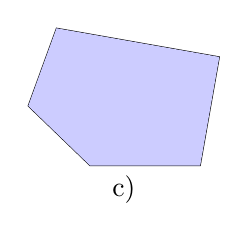
\begin{tikzpicture}[scale=.7]
			\draw (0,0)coordinate (A) --++(2,0) coordinate (B)--++(80:2)coordinate (C)--++(170:3)coordinate (D)--++(-110:1.5)coordinate (E)--cycle;
			\fill[blue!20] (A)--(B)--(C)--(D)--(E)--cycle;
			%	\foreach \x/\g in {A/90,B/180,C/-45,D/0,E/0}
			%			\fill[black] 	(\x) circle (1pt)
			%			($(\g:3mm)+(\x)$) node {$\x$};
			\path (current bounding box.south) node[below]{c)};
		\end{tikzpicture}
		\begin{tikzpicture}
			\def\a{.8}
			\draw (0:0)coordinate (N)
			--(22.5:\a)coordinate (P)
			--++(67.5:\a)coordinate (Q)--++(112.5:\a) coordinate (S)--++(157.5:\a) coordinate (R)
			--++(202.5:\a) coordinate (X)
			--++(247.5:\a) coordinate (Y)
			--++(292.5:\a) coordinate (Z)
			--cycle;
			\fill[green!50!yellow] (N)--(P)--(Q)--(S)--(R)--(X)--(Y)--(Z)--cycle;
			\draw
			pic[draw,angle radius=2mm]{ angle=S--Q--P}
			pic[draw,angle radius=2mm]{ angle=Q--P--N}
			pic[draw,angle radius=2mm]{ angle=P--N--Z}
			pic[draw,angle radius=2mm]{ angle=X--R--S}
			pic[draw,angle radius=2mm]{ angle=R--S--Q}
			pic[draw,angle radius=2mm]{ angle=N--Z--Y}
			pic[draw,angle radius=2mm]{ angle=Z--Y--X}
			pic[draw,angle radius=2mm]{ angle=Y--X--R}
			;
			\path (S)--(R) node[midway,sloped,scale=0.5]{$|$}
			(S)--(Q) node[midway,sloped,scale=0.5]{$|$}
			(Q)--(P) node[midway,sloped,scale=0.5]{$|$}
			(P)--(N) node[midway,sloped,scale=0.5]{$|$}
			(N)--(Z) node[midway,sloped,scale=0.5]{$|$}
			(Z)--(Y) node[midway,sloped,scale=0.5]{$|$}
			(Y)--(X) node[midway,sloped,scale=0.5]{$|$}
			(R)--(X) node[midway,sloped,scale=0.5]{$|$};
%					\foreach \x/\g in {N/180,P/180,Q/-90,S/0,R/0,X/0,Y/0,Z/0}
%					\fill[black] 	(\x) circle (1.5pt)
%					($(\g:3mm)+(\x)$) node {$\x$};
			\path (current bounding box.south) node[below]{d)};
		\end{tikzpicture}
		\begin{tikzpicture}
			\def\a{2} %cạnh
			\path (0:0) coordinate (B)
			++(0:\a) coordinate (C)
			++(90:\a) coordinate (D)
			++(180:\a) coordinate (A);
			\draw (A)--(B)--(C)--(D)--cycle;
			\fill[blue!60] (A)--(B)--(C)--(D)--cycle;
			\path
			(A)--(B) node[midway,sloped,scale=0.5]{$|$}
			(B)--(C) node[midway,sloped,scale=0.5]{$|$}
			(C)--(D) node[midway,sloped,scale=0.5]{$|$}
			(D)--(A) node[midway,sloped,scale=0.5]{$|$};
			\draw 
			pic[draw,angle radius=2mm]{right angle=D--C--B}
			pic[draw,angle radius=2mm]{right angle=C--B--A}
			pic[draw,angle radius=2mm]{right angle=B--A--D}
			pic[draw,angle radius=2mm]{right angle=A--D--C}
			;
			%	\foreach \x/ \goc in {A/135,B/-135,C/-45,D/45} 
			%	\fill (\x) circle (1pt)
			%	($(\x)+(\goc:3mm)$) node {$\x$};
			\path (current bounding box.south) node[below]{e)};
		\end{tikzpicture}
		\begin{tikzpicture}
			\def\a{1.2}
			\draw (0:0)coordinate (N)
			--(-90:\a)coordinate (P)
			--++(-30:\a)coordinate (Q)--++(30:\a) coordinate (S)--++(90:\a) coordinate (R)--++(150:\a) coordinate (M)
			--cycle;
			\fill[green!50] (M)--(N)--(P)--(Q)--(S)--(R)--cycle;
			\path
			(M)--(N) node[midway,sloped,scale=0.5]{$|$}
			(N)--(P) node[midway,sloped,scale=0.5]{$|$}
			(P)--(Q) node[midway,sloped,scale=0.5]{$|$}
			(Q)--(S) node[midway,sloped,scale=0.5]{$|$}
			(S)--(R) node[midway,sloped,scale=0.5]{$|$}
			(R)--(M) node[midway,sloped,scale=0.5]{$|$}
			;
			\draw pic[draw,,angle radius=2mm]{angle=N--M--R}
			pic[draw,,angle radius=2mm]{angle=M--R--S}
			pic[draw,,angle radius=2mm]{angle=R--S--Q}
			pic[draw,,angle radius=2mm]{angle=S--Q--P}
			pic[draw,,angle radius=2mm]{angle=Q--P--N}
			pic[draw,,angle radius=2mm]{angle=P--N--M}
			;
			%	\foreach \x/\g in {N/180,P/180,Q/-90,S/0,R/0,M/90}
			%	\fill[black] 	(\x) circle (1.5pt)
			%	($(\g:3mm)+(\x)$) node {$\x$};
			\path (current bounding box.south) node[below]{g)};
		\end{tikzpicture} 
	\end{center}
	\loigiai{
		Ta có Hình b) là ngũ giác đều; Hình d) là bát giác đều; Hình e) là tứ giác đều; Hình g) là lục giác đều. \\
		Các Hình a) và Hình c) không phải là đa giác đều.
	}
\end{vd}

\begin{vd}%[SGK CD Toán 9]%[Dự án EX-9-Đề Cương Toán 9]%[Nguyễn Tiến Liên]%[9H3H3-1]
	Tính số đo mỗi góc của một ngũ giác đều.
	\loigiai{
		\immini{
			Xét ngũ giác đều $ABCDE$ (hình bên), ta thấy: Tổng $5$ góc của ngũ giác đều đó bằng tổng các góc trong ba tam giác $ABC$, $ACD$, $ADE$, tức là bằng $3\cdot 180^\circ = 540^\circ$.\\
			Do tất cả các góc của ngũ giác đều bằng nhau nên số đo mỗi góc của ngũ giác đều bằng $\dfrac{540^\circ}{5} = 108^\circ$.
		}{
			\begin{tikzpicture}[>=stealth,line join=round,line cap=round,font=\footnotesize,scale=1]
				\path 
				(0,1.5) coordinate (O)
				($ (O) + (90:1.5) $) coordinate (A) 
				($ (O) + (18:1.5) $) coordinate (B) 
				($ (O) + (-54:1.5) $) coordinate (C) 
				($ (O) + (-126:1.5) $) coordinate (D) 
				($ (O) + (-198:1.5) $) coordinate (E)
				;
				\draw (A)--(B)--(C)--(D)--(E)--cycle;
				\draw[red] (D)--(A)--(C);
				\foreach \l/\g in {A/90,B/0,C/-45,D/-135,E/180}
				\draw[fill=black] (\l) circle (1pt) +(\g:.3) node{$\l$};
			\end{tikzpicture}
		}
	}
\end{vd}

\begin{vd}%[SBT CTST Toán 9]%[Dự án EX-9-Đề Cương Toán 9]%[Nguyễn Tiến Liên]%[9H3V3-1]
	Cho đường tròn $(O;R)$. Lấy các điểm $A$, $B$, $C$, $D$, $E$, $F$ trên đường tròn $(O;R)$ sao cho số đo các cung $\wideparen{AB}$, $\wideparen{BC}$, $\wideparen{CD}$, $\wideparen{DE}$, $\wideparen{EF}$, $\wideparen{FA}$ bằng nhau. Đa giác $ABCDEF$ có là đa giác đều không? Vì sao?
	\loigiai{
		\immini{
			Các cung $\wideparen{AB}$, $\wideparen{BC}$, $\wideparen{CD}$, $\wideparen{DE}$, $\wideparen{EF}$, $\wideparen{FA}$ chia đường tròn $(O;R)$ thành sáu cung có số đo bằng nhau, suy ra mỗi cung có số đo bằng $\dfrac{360^\circ}{6}=60^\circ$. \\
			Ta có $\widehat{AOB}$ là góc ở tâm chắn cung $AB$, $\widehat{BOC}$ là góc ở tâm chắn cung $BC$. \\
			Suy ra $\widehat{AOB}=\text{sđ}\wideparen{AB}=60^\circ$, $\widehat{BOC}=\text{sđ}\wideparen{BC}=60^\circ$. \\
			Xét tam giác $OAB$, ta có: $OA=OB=R$; $\widehat{AOB}=60^\circ$.\\
			Suy ra tam giác $OAB$ đều, do đó $AB=OA=R$ và $\widehat{ABO}=60^\circ$.\quad $(1)$\\
			Tương tự, tam giác $BOC$ có $OB=OC=R$ và $\widehat{BOC}=60^\circ$. \\
			Suy ra tam giác $OBC$ đều, do đó $BC=OB=R$ và $\widehat{OBC}=60^\circ$. \quad $(2)$
		}
		{
			\begin{tikzpicture}
				\def\r{2}
				\path (0:0) coordinate (O) 
				(30:\r) coordinate (B)
				(90:\r) coordinate (A)
				(-30:\r) coordinate (C)
				(-90:\r) coordinate (D)
				(150:\r) coordinate (F)
				(-150:\r) coordinate (E);
				\draw
				(O) circle (\r)
				(A)--(B)--(C)--(D)--(E)--(F)--cycle
				;
				\draw[red] (A)--(D) (B)--(E) (C)--(F);
				\foreach \x/\g in {A/90,B/30,C/-30,D/-90,E/-150,F/150}
				\fill[black] (\x) circle(1pt)
				($(\g:3mm)+(\x)$) node {$\x$};
				\fill[black] (O) circle(1pt)
				($(180:5mm)+(O)$) node {$O$};
			\end{tikzpicture}	
		}
		Từ $(1)$ và $(2)$ suy ra $AB=BC=R$ và $\widehat{ABC}=\widehat{ABO}+\widehat{OBC}=60^\circ+60^\circ=120^\circ$. \\
		Chứng minh tương tự, ta có đa giác $ABCDEF$ có các cạnh đều bằng $R$ và các góc đều bằng $120^\circ$. \\
		Vậy $ABCDEF$ là một đa giác đều.
	}
\end{vd}

\begin{bt}%[SBT KNTT Toán 9]%[Dự án EX-9-Đề Cương Toán 9]%[Nguyễn Tiến Liên]%[9H3N3-1]
	Hình phẳng nào dưới đây có dạng đa giác đều?
	\begin{center}
		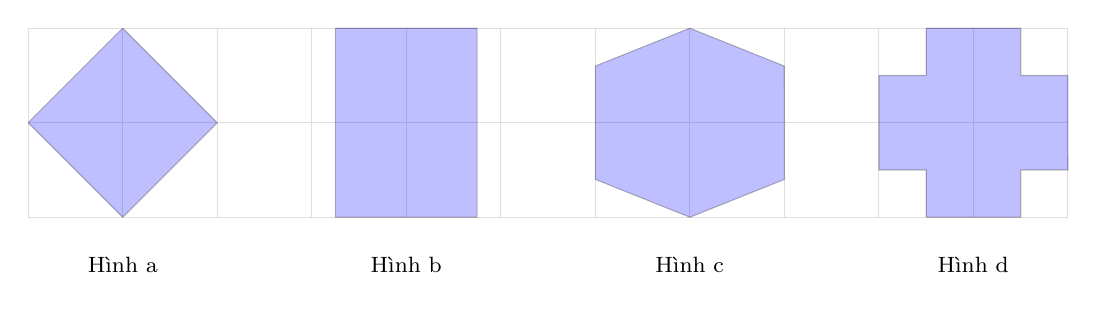
\begin{tikzpicture}[>=stealth,line join=round,line cap=round,font=\footnotesize,scale=1.2]	
			\node at (0,-1.5) {Hình a};
			\node at (3,-1.5) {Hình b};
			\node at (6,-1.5) {Hình c};
			\node at (9,-1.5) {Hình d};
			\draw[gray!25] (-1,-1) grid (10,1);
			%Hình vuông
			\path (0,0) coordinate (O1)++(0:1) coordinate (A)	
			(90:1) coordinate (B)
			(180:1) coordinate (C)
			(270:1) coordinate (D);
			\draw[fill=blue,opacity=0.25] (A)--(B)--(C)--(D)--cycle;
			%Hình chữ nhật
			\path (3,0) coordinate (O2)++(.75,1) coordinate (M)	
			(O2)++(-.75,1) coordinate (N)
			(O2)++(-.75,-1) coordinate (P)
			(O2)++(.75,-1) coordinate (Q);
			\draw[fill=blue,opacity=0.25] (M)--(N)--(P)--(Q)--cycle;
			%Hình lục giác 
			\path (6,0) coordinate (O3)++(1,.6) coordinate (E)	
			(O3)++(0,1) coordinate (F)
			(O3)++(-1,.6) coordinate (G)
			(O3)++(-1,-.6) coordinate (H)
			(O3)++(0,-1) coordinate (I)
			(O3)++(1,-.6) coordinate (K);
			\draw[fill=blue,opacity=0.25]  (E)--(F)--(G)--(H)--(I)--(K)--cycle;
			%Hình chữ thập
			\path (9,0) coordinate (O4)++(1,.5) coordinate (A1)	
			(O4)++(0.5,.5) coordinate (A2)
			(O4)++(.5,1) coordinate (A3)
			(O4)++(-.5,1) coordinate (A4)
			(O4)++(-.5,.5) coordinate (A5)
			(O4)++(-1,.5) coordinate (A6)
			(O4)++(-1,-.5) coordinate (A7)
			(O4)++(-.5,-.5) coordinate (A8)
			(O4)++(-.5,-1) coordinate (A9)
			(O4)++(.5,-1) coordinate (A10)
			(O4)++(.5,-.5) coordinate (A11)
			(O4)++(1,-.5) coordinate (A12);
			\draw[fill=blue,opacity=0.25]  (A1)--(A2)--(A3)--(A4)--(A5)--(A6)--(A7)--(A8)--(A9)--(A10)--(A11)--(A12)--cycle;
		\end{tikzpicture}
	\end{center}
	\loigiai{
		Hình a là hình vuông nên là hình có dạng đa giác đều.
	}
\end{bt}

\begin{bt}%[Dự án EX-9-Đề Cương Toán 9]%[Nguyễn Tiến Liên]%[9H3N3-1]
	Trong các hình phẳng dưới đây, hình phẳng nào là đa giác đều?
	\begin{center}
		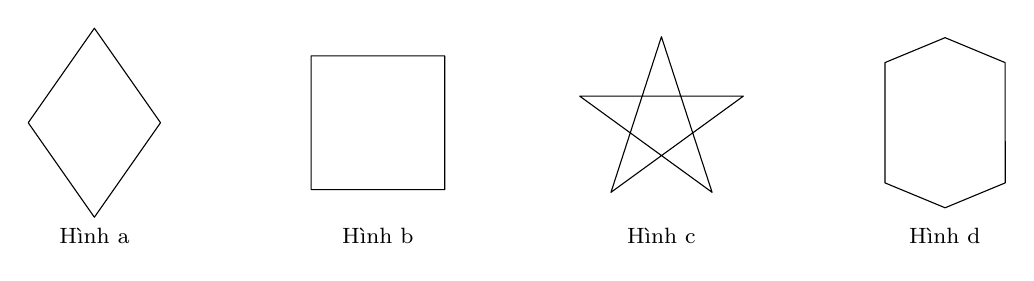
\begin{tikzpicture}[>=stealth,line join=round,line cap=round,font=\footnotesize,scale=1.2]	
			\node at (0,-1.2) {Hình a};
			\node at (3,-1.2) {Hình b};
			\node at (6,-1.2) {Hình c};
			\node at (9,-1.2) {Hình d};
			%Hình tứ giác
			\path (0,0) coordinate (O1)++(90:1) coordinate (A)	
			(O1)++(0:0.7) coordinate (B)
			(O1)++(-90:1) coordinate (C)
			(O1)++(180:0.7) coordinate (D);
			\draw (A)--(B)--(C)--(D)--cycle;
			%Hình vuông
			\path (3,0) coordinate (O2)++(45:1) coordinate (M)	
			(O2)++(135:1) coordinate (N)
			(O2)++(-135:1) coordinate (P)
			(O2)++(-45:1) coordinate (Q);
			\draw (M)--(N)--(P)--(Q)--(M);
			%Hình ngôi sao 5 cánh
			\path (6,0) coordinate (O3)++(90:.91) coordinate (E)	
			(O3)++(162:.91) coordinate (F)
			(O3)++(234:.91) coordinate (G)
			(O3)++(306:.91) coordinate (H)
			(O3)++(18:.91) coordinate (I);
			\draw (E)--(H)--(F)--(I)--(G)--cycle;
			%Hình lục giác
			\path (9,0) coordinate (O4)++(45:.9) coordinate (A1)	
			(O4)++(90:.9) coordinate (A2)
			(O4)++(135:.9) coordinate (A3)
			(O4)++(225:.9) coordinate (A4)
			(O4)++(270:.9) coordinate (A5)
			(O4)++(315:.9) coordinate (A6);
			\draw (A1)--(A2)--(A3)--(A4)--(A5)--(A6)--cycle;
		\end{tikzpicture}
	\end{center}
	\loigiai{
		Trong các hình phẳng trên, hình b là hình tứ giác đều (Hình vuông).
	}
\end{bt}

\begin{bt}%[Dự án EX-9-Đề Cương Toán 9]%[Nguyễn Tiến Liên]%[9H3N3-1]
	Những hình nào dưới đây là đa giác đều?
	\begin{multicols}{2}
		\begin{enumerate}
			\item Tam giác đều.
			\item Hình vuông.
			\item Hình tròn.
			\item Hình bình hành.
			\item Hình chữ nhật.
			\item Lục giác đều.
		\end{enumerate}
	\end{multicols}
	\loigiai{
		\begin{itemize}
			\item Tam giác đều, hình vuông và lục giác đều là các đa giác đều.
			\item Hình tròn, hình bình hành và hình chữ nhật, không phải là đa giác đều.
		\end{itemize}
	}
\end{bt}

\begin{bt}%[SGK KNTT Toán 9]%[Dự án EX-9-Đề Cương Toán 9]%[Nguyễn Tiến Liên]%[9H3H3-1]
	\immini{
		Cho một bát giác đều (đa giác đều $8$ cạnh) nội tiếp một đường tròn tâm $O$ (Hình bên). Hỏi mỗi góc của bát giác đều có số đo bằng bao nhiêu?
	}{
		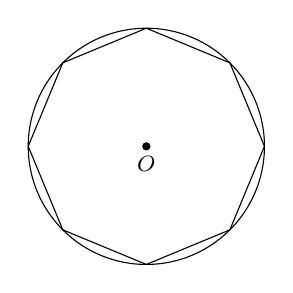
\begin{tikzpicture}[>=stealth,line join=round,line cap=round,font=\footnotesize,scale=1]
			\def\R{1.5}
			\draw circle (\R cm);
			\foreach \i in {0,...,7}{
				\coordinate (A\i) at (360*\i/8:\R cm);	
			}
			\draw (A0)--(A1)--(A2)--(A3)--(A4)--(A5)--(A6)--(A7)--cycle;
			\fill[black] circle (1.5pt) node[below]{$O$};	
		\end{tikzpicture}
	}
	\loigiai{
		\immini{
			Vì bát giác đều nên $\widehat{A_1OA_2}=\widehat{A_2OA_3}=\dfrac{360^\circ}{8}=45^\circ$.\\
			Tam giác $OA_1A_2$ cân tại $O$ nên $$\widehat{OA_2A_1}=\dfrac{180^\circ-\widehat{A_1OA_2}}{2}=\dfrac{180^\circ-45^\circ}{2}=67{,}5^\circ.$$
			Tương tự ta có $\widehat{OA_2A_3}=67{,}5^\circ$.\\
			Do đó $\widehat{A_1A_2A_3} = \widehat{OA_2A_1} + \widehat{OA_2A_3} = 67{,}5^\circ + 67{,}5^\circ = 135^\circ$.\\
			Vậy mỗi góc của bát giác đều có số đo $135^\circ$.
			
		}{
			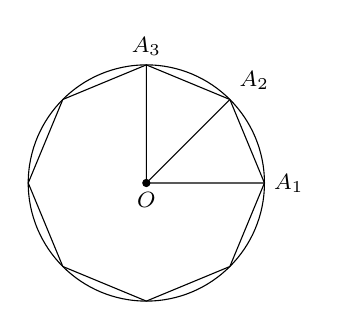
\begin{tikzpicture}[>=stealth,line join=round,line cap=round,font=\footnotesize,scale=1]
				\def\R{1.5}
				\draw circle (\R cm);
				\foreach \i in {0,...,7}{
					\coordinate (A\i) at (360*\i/8:\R cm);	
				}
				\draw (A0)--(A1)--(A2)--(A3)--(A4)--(A5)--(A6)--(A7)--cycle;
				\fill[black] circle (1.5pt) node[below]{$O$};
				\draw (A1)node[above right]{$A_2$}--(0,0)--(A0)node[right]{$A_1$} (0,0)--(A2) node[above]{$A_3$};	
			\end{tikzpicture}
		}
	}
\end{bt}

\begin{bt}%[Dự án EX-9-Đề Cương Toán 9]%[Nguyễn Tiến Liên]%[9H3H3-1]
	Mỗi góc của một đa giác đều bằng bao nhiêu độ? Biết đa giác đó là
	\begin{multicols}{3}
		\begin{enumerate}
			\item Ngũ giác đều.
			\item Lục giác đều.
			\item Bát giác đều.
		\end{enumerate}
	\end{multicols}
	\loigiai{
		Số đo mỗi góc của đa giác đều $n$ cạnh ($n\in \mathbb{N}$, $n \ge 3$) được tính bằng công thức $\dfrac{(n-2)\cdot 180^\circ}{n}$.\\
		Do đó
		\begin{enumerate}
			\item Mỗi góc trong ngũ giác đều bằng $\dfrac{(5-2)\cdot 180^\circ}{5} = 108^\circ$.
			\item Mỗi góc trong lục giác đều bằng $\dfrac{(6-2)\cdot 180^\circ}{6} = 120^\circ$.
			\item Mỗi góc trong bát giác đều bằng $\dfrac{(8-2)\cdot 180^\circ}{8} = 135^\circ$.
		\end{enumerate}
	}
\end{bt}

\begin{bt}%[SBT CTST Toán 9]%[Dự án EX-9-Đề Cương Toán 9]%[Nguyễn Tiến Liên]%[9H3V3-1]
	Cho đường tròn $(O;R)$, trên đó lấy các điểm $M$, $N$, $P$, $Q$, $R$ sao cho số đo các cung $\wideparen{MN}$, $\wideparen{NP}$, $\wideparen{PQ}$, $\wideparen{QR}$, $\wideparen{RM}$ bằng nhau. Đa giác $MNPQR$ có là đa giác đều không? Vì sao?
	\loigiai{
		\immini{
			Các cung $\wideparen{MN}$, $\wideparen{NP}$, $\wideparen{PQ}$, $\wideparen{QR}$, $\wideparen{RM}$ chia đường tròn $(O;R)$ thành năm cung có số đo bằng nhau, suy ra mỗi cung có số đo bằng $\dfrac{360^\circ}{5}=72^\circ$. \\
			Ta có $\widehat{MON}$ là góc ở tâm chắn cung $MN$, $\widehat{NOP}$ là góc ở tâm chắn cung $NP$.
			\\ 
			Suy ra $\widehat{MON}=\text{sđ}\wideparen{MN}=72^\circ$, $\widehat{NOP}=\text{sđ}\wideparen{NP}=72^\circ$  \\
			Xét tam giác $OMN$, ta có $OM=ON$ và  $\widehat{ONM}=\dfrac{180^\circ-\widehat{MON}}{2}=54^\circ$. \\
			Xét tam giác $ONP$, ta có $ON=OP$ và $\widehat{ONP}=54^\circ$. 
		}
		{
			\begin{tikzpicture}
				\def\r{2}
				\path (0:0) coordinate (O) 
				(90:\r) coordinate (M)
				(18:\r) coordinate (N)
				(-54:\r) coordinate (P)
				(-126:\r) coordinate (Q)
				(162:\r) coordinate (R);
				\draw
				(O) circle (\r)
				(M)--(N)--(P)--(Q)--(R)--cycle
				;
				\draw[red] 
				(O)--(M)
				(O)--(N)
				(O)--(P)
				(O)--(Q)
				(O)--(R)
				;
				\foreach \x/\g in {M/90,N/30,P/-45,Q/-135,R/150,O/-90}
				\fill[black] 	(\x) circle(1pt)
				($(\g:3mm)+(\x)$) node {$\x$};
			\end{tikzpicture}	
		}
		Xét $\triangle OMN$ và $\triangle ONP$, ta có
		\begin{itemize}
			\item $OM=OP$ ($=R$).
			\item $\widehat{MON} = \widehat{NOP} = 72^\circ$.
			\item $ON$ cạnh chung.
		\end{itemize}
		Suy ra $\triangle OMN=\triangle ONP$ (c.g.c) nên $MN=NP$ và $\widehat{MNP}=\widehat{ONM}+\widehat{ONP}=54^\circ+54^\circ=108^\circ$. \\
		Chứng minh tương tự, ta có đa giác $MNPQR$ có các cạnh bằng nhau và các góc đều bằng $108^\circ$.\\
		Vậy $MNPQR$ là một đa giác đều.
	}
\end{bt}

\begin{bt}%[SGK KNTT Toán 9]%[Dự án EX-9-Đề Cương Toán 9]%[Nguyễn Tiến Liên]%[9H3V3-1]
	\immini{
		Cho tam giác đều $ABC$ có cạnh $6$ cm. Trên cạnh $AB$ lấy các điểm $M$, $N$; trên cạnh $BC$ lấy các điểm $P$, $Q$; trên cạnh $CA$ lấy các điểm $E$, $F$, sao cho các đoạn thẳng $AM$, $MN$, $NB$, $BP$, $PQ$, $QC$, $CE$, $EF$, $FA$ đều bằng $2$ cm như hình bên. Hỏi $MNPQEF$ có là một lục giác đều hay không?
	}{\vspace*{-6mm}
		\begin{tikzpicture}[line join = round, line cap = round,>=stealth,font=\footnotesize,scale=1] 
			\def\a{3}
			\def\goc{60}
			\coordinate[label = left:$B$] (B) at (0,0); 
			\coordinate[label = right:$C$] (C) at ($(B)+(\a,0)$); 
			\coordinate[label = above:$A$] (A) at ($(B)+(\goc:\a)$);
			\coordinate[label = left:$B$] (B) at (0,0); 
			\coordinate[label = left:$M$] (M) at ($(A)!1/3!(B)$);
			\coordinate[label = left:$N$] (N) at ($(B)!1/3!(A)$);
			\coordinate[label = right:$F$] (F) at ($(A)!1/3!(C)$);
			\coordinate[label = right:$E$] (E) at ($(C)!1/3!(A)$);
			\coordinate[label = below:$Q$] (Q) at ($(C)!1/3!(B)$);
			\coordinate[label = below:$P$] (P) at ($(B)!1/3!(C)$);
			
			\draw (A)--(B)--(C)--cycle;
			\draw (M)--(F) (E)--(Q) (N)--(P); 
			\foreach \x in {A,B,C,M,F,E,Q,P,N} \fill[black] (\x) circle (1pt);
			\foreach \dau/\cuoi in {A/M,M/N,N/B,B/P,P/Q,Q/C,C/E,E/F,F/A} \draw (\dau)--(\cuoi) node[midway,sloped] {\tiny $|$}; 
		\end{tikzpicture}
	}
	\loigiai{
		Theo hình vẽ, ta thấy $MNPQEF$ là một đa giác lồi.\\
		Ta có $\dfrac{AM}{AB}=\dfrac{AF}{AC}=\dfrac{1}{3}$.\\
		Theo định lí Thalès đảo cho tam giác $ABC$ và đường thẳng $MF$ thì $MF\parallel BC$.\\
		Suy ra $\dfrac{MF}{BC}=\dfrac{AM}{AB}=\dfrac{1}{3}$.\\
		Do đó $MF=\dfrac{BC}{3}=2$ cm.\\
		Tương tự, $NP=QE=2$ cm.\\
		Vậy lục giác $MNPQEF$ có tất cả các cạnh bằng nhau.\\
		Mặt khác, tam giác $AMF$ là tam giác đều vì $AM=MF=FA=2$ cm nên
		$$
		\widehat{FMA}=60^{\circ} \text { và } \widehat{FMN}=180^{\circ}-\widehat{FMA}=120^{\circ} .
		$$
		Tương tự các góc tại các đỉnh $N$, $P$, $Q$, $E$, $F$ của lục giác $MNPQEF$ đều bằng nhau và bằng $120^{\circ}$.\\
		Do đó, lục giác $MNPQEF$ có các cạnh và các góc bằng nhau.\\
		Vậy $MNPQEF$ là lục giác đều.
	}
\end{bt}

\begin{bt}%[Dự án EX-9-Đề Cương Toán 9]%[Nguyễn Tiến Liên]%[9H3V3-1]
	Cho tam giác đều $ABC$. Trên cạnh $AB$ lấy các điểm $M$, $N$ sao cho $AM = MN = NB$. Trên cạnh $AC$ lấy các điểm $D$, $E$ sao cho $AD = DE = EC$. Trên cạnh $BC$ lấy các điểm $P$, $Q$ sao cho $BP = PQ = PC$. Chứng minh $MDEQPN$ là lục giác đều.
	\loigiai{
		\begin{center}
			\begin{tikzpicture}[>=stealth,line join=round,line cap=round,font=\footnotesize,scale=1.5]	
				%Hình tam giác đều
				\path (0,0) coordinate (O)++(90:1) coordinate (A)	
				(-30:1) coordinate (C)
				(-150:1) coordinate (B)
				($(A)!.3333!(B)$)coordinate (M)
				($(A)!.6666!(B)$)coordinate (N)
				($(A)!.3333!(C)$)coordinate (D)
				($(A)!.6666!(C)$)coordinate (E)
				($(B)!.3333!(C)$)coordinate (P)
				($(B)!.6666!(C)$)coordinate (Q)
				;
				\draw (A)--(C)--(B)--cycle (N)--(P)(Q)--(E)(M)--(D);
				\foreach \t/\g in {A/90,B/-90,C/-90,M/130,N/130,D/70,E/70,P/-90,Q/-90}{
					\draw[fill=black] (\t) circle (1pt) node[shift={(\g:7pt)},font=\scriptsize]{$ \t $};}
			\end{tikzpicture}
		\end{center}
		Ta có các tam giác $AMD$, $BNP$, $CQE$ là tam giác đều có cạnh bằng nhau.\\
		Suy ra $MD = DE = EQ = QP = PN$. $\quad (1)$\\
		Lại có $\widehat{AMD} = \widehat{ADM}=\widehat{CEQ} = \widehat{CQE}=\widehat{BPN} = \widehat{BNP} = 60^\circ$.\\
		Suy ra $\widehat{NMD} = \widehat{EDM} =\widehat{DEQ} = \widehat{EQP}= \widehat{QPN} = \widehat{PNM} = 120^\circ$. $\quad (2)$\\
		Từ $(1)$ và $(2)$ suy ra $MDEQPN$ là lục giác đều.
	}
\end{bt}

\begin{bt}%[Dự án EX-9-Đề Cương Toán 9]%[Nguyễn Tiến Liên]%[9H3V3-1]
	Cho hình thoi $ABCD$ có $\widehat{A} = 120^\circ$. Gọi $M$, $N$, $P$, $Q$ lần lượt là trung điểm của $AB$, $BC$, $CD$, $DA$. Chứng minh $AMNCPQ$ là lục giác đều.
	\loigiai{
		\begin{center}
			\begin{tikzpicture}[>=stealth,line join=round,line cap=round,font=\footnotesize,scale=1.5]	
				\path (0,0) coordinate (O1)++(90:1) coordinate (A)	
				(0:2) coordinate (D)
				(-90:1) coordinate (C)
				(180:2) coordinate (B)
				($(A)!.5!(B)$)coordinate (M)
				($(B)!.5!(C)$)coordinate (N)
				($(C)!.5!(D)$)coordinate (P)
				($(D)!.5!(A)$)coordinate (Q);
				\draw (A)--(B)--(C)--(D)--cycle(M)--(N)(P)--(Q)(A)--(C)(B)--(D);	
				\foreach \x/\y in {A/M,B/M,A/Q,D/Q,C/P,D/P,B/N,C/N}{
					\path (\x)--(\y) node[midway,sloped]{$|$};
				}
				\foreach \t/\g in {A/90,B/-90,C/-90,M/130,N/-90,D/70,P/-90,Q/90}{
					\draw[fill=black] (\t) circle (.6pt) node[shift={(\g:7pt)},font=\scriptsize]{$\t$};}
			\end{tikzpicture}
		\end{center}
		Tứ giác $ABCD$ là hình thoi nên $AC$ là phân giác của $\widehat{A}$ hay $\widehat{BAC} =\widehat{DAC}= 60^\circ$.\\
		Do vậy $\triangle ABC$ và $\triangle ADC$ là các tam giác đều.\\
		Ta có $M$, $N$, $P$, $Q$ lần lượt là trung điểm của $AB$, $BC$, $CD$, $DA$\\
		nên $MN$ và $PQ$ lần lượt là đường trung bình của $\triangle ABC$ và $\triangle ADC$.\\
		Suy ra $MN=PQ=\dfrac{AC}{2}$ (theo định lý đường trung bình của tam giác).\\
		Do đó  $AM=MN=NC=CP=PQ=QA$. $\quad (1)$\\
		Hình thoi $ABCD$ có $\widehat{A} = 120^\circ$ nên $\widehat{BAD}=\widehat{BCD}= 120^\circ$ hay $\widehat{MAQ}=\widehat{PCN}= 120^\circ$.\\
		Lại có $\widehat{BMN} = \widehat{BNM}=\widehat{DQP} = \widehat{DPQ} = 60^\circ$.\\ 
		Suy ra $\widehat{NMA} = \widehat{CNM} =\widehat{AQP} = \widehat{QPC}= 120^\circ$.\\
		Do đó $\widehat{MAQ} = \widehat{AQP} =\widehat{QPC} = \widehat{PCN}= \widehat{CNM} = \widehat{NMA} = 120^\circ$. $\quad (2)$\\
		Từ $(1)$ và $(2)$ suy ra $AMNCPQ$ là lục giác đều.
	}
\end{bt}

\begin{bt}%[SGK KNTT Toán 9]%[Dự án EX-9-Đề Cương Toán 9]%[Nguyễn Tiến Liên]%[9H3V3-1]
	\immini{
		Cho $M$, $N$, $P$, $Q$, $K$ lần lượt là trung điểm của các cạnh $AB$, $BC$, $CD$, $DE$ và $EA$ của ngũ giác đều $ABCDE$ (hình bên). Hỏi $MNPQK$ có phải là ngũ giác đều hay không?	
	}{
		\begin{tikzpicture}[line join = round, line cap = round,>=stealth,font=\footnotesize,scale=1] 
			\def\a{2}
			\coordinate[label = below:$D$] (D) at (0,0); 
			\coordinate[label = below:$C$] (C) at ($(D)+(\a,0)$);
			\coordinate[label = right:$B$] (B) at ($(C)!1!-108:(D)$);
			\coordinate[label = above:$A$] (A) at ($(B)!1!-108:(C)$);
			\coordinate[label = left:$E$] (E) at ($(A)!1!-108:(B)$);
			
			\coordinate[label = below:$P$] (P) at ($(D)!1/2!(C)$);
			\coordinate[label = right:$N$] (N) at ($(C)!1/2!(B)$);
			\coordinate[label = above right:$M$] (M) at ($(B)!1/2!(A)$);
			\coordinate[label = above left:$K$] (K) at ($(A)!1/2!(E)$);
			\coordinate[label = left:$Q$] (Q) at ($(E)!1/2!(D)$);
			\draw (D)--(C)--(B)--(A)--(E)--cycle;
			\draw (M)--(N)--(P)--(Q)--(K)--cycle; 
			\foreach \x in {D,C,B,A,E,M,N,P,Q,K} \fill[black] (\x) circle (1pt);
			\foreach \dau/\cuoi in {A/K,K/E,E/Q,Q/D,D/P,P/C,C/N,N/B,B/M,M/A} \draw (\dau)--(\cuoi) node[midway,sloped] {\tiny $|$}; 
		\end{tikzpicture}
	}	
	\loigiai{
		Vì $ABCDE$ là ngũ giác đều nên $AB=BC=CD=DE=EA$ và $\widehat{A}=\widehat{B}=\widehat{C}=\widehat{D}=\widehat{E}$.\\
		Suy ra $\triangle AEB=\triangle BAC=\triangle CBD=\triangle DCE=\triangle EDA$ (c.g.c).\\
		Do đó $EB=AC=BD=CE=DA$.\hfill $(1)$\\
		Xét $\triangle AEB$, ta có 
		\begin{itemize}
			\item $K$ là trung điểm của $AE$.
			\item $M$ là trung điểm của $AB$.
		\end{itemize}
		Do đó $KM$ là đường trung bình của $\triangle AEB$.\\
		Suy ra $KM=\dfrac{1}{2}EB$.\hfill $(2)$\\
		Tương tự, ta chứng minh được
		$MN=\dfrac{1}{2}AC$; $NP=\dfrac{1}{2}BD$; $PQ=\dfrac{1}{2}CE$; $QK=\dfrac{1}{2}DA$. \hfill $(3)$\\
		Từ $(1)$, $(2)$ và $(3)$, suy ra $KM=MN=NP=PQ=QK$, do đó ngũ giác $MNPQK$ có tất cả các cạnh bằng nhau.\\
		Dễ thấy $\triangle AKM=\triangle BMN=\triangle CNP=\triangle DPQ=\triangle EQK$ (c.g.c), kết hợp mỗi tam giác đó cân nên suy ra 
		$$\widehat{AKM}=\widehat{AMK}=\widehat{BMN}=\widehat{BNM}=\widehat{CNP}=\widehat{CPN}=\widehat{DPQ}=\widehat{DQP}=\widehat{EQK}=\widehat{EKQ}.$$
		Do đó $\widehat{QKM}=\widehat{KMN}=\widehat{MNP}=\widehat{NPQ}=\widehat{PQK}$, hay ngũ giác $MNPQK$ có tất cả các góc tại các đỉnh $M$, $N$, $P$, $Q$, $K$ bằng nhau.\\
		Vậy ngũ giác $MNPQK$ có các cạnh và các góc bằng nhau nên nó là ngũ giác đều.
	}
\end{bt}

\begin{bt}%[SGK CTST Toán 9]%[Dự án EX-9-Đề Cương Toán 9]%[Nguyễn Tiến Liên]%[9H3V3-1]
	Cho lục giác đều $ABCDEF$ có $M$, $N$, $P$, $Q$, $R$, $S$ lần lượt là trung điểm của các cạnh $AB$, $BC$, $CD$, $DE$, $EF$, $FA$. Đa giác $MNPQRS$ có là đa giác đều không? Vì sao?
	\loigiai{
		\begin{center}
			\begin{tikzpicture}[line join = round, line cap = round,>=stealth,font=\footnotesize,scale=1] 
				\def\r{2}
				\path (0:0) coordinate (O) 
				(30:\r) coordinate (B)
				(90:\r) coordinate (A)
				(-30:\r) coordinate (C)
				(-90:\r) coordinate (D)
				(150:\r) coordinate (F)
				(-150:\r) coordinate (E)
				($(A)!.5!(B)$) coordinate (M)
				($(B)!.5!(C)$) coordinate (N)
				($(C)!.5!(D)$) coordinate (P)
				($(D)!.5!(E)$) coordinate (Q)
				($(E)!.5!(F)$) coordinate (R)
				($(F)!.5!(A)$) coordinate (S)		
				;
				\draw
				(A)--(B)--(C)--(D)--(E)--(F)--cycle
				(M)--(N)--(P)--(Q)--(R)--(S)--cycle
				;
				\foreach \x/\g in {A/90,B/30,C/-30,D/-90,E/-150,F/150,M/30,N/0,P/-30,Q/-150,R/180,S/150}
				\fill[black] 	(\x) circle(1.5pt)
				($(\g:3mm)+(\x)$) node {$\x$};
			\end{tikzpicture}	 
		\end{center}
		\begin{itemize}
			\item Chứng minh các cạnh của đa giác bằng nhau. \\
			Do $ABCDEF$ là lục giác đều nên ta có các cạnh đều bằng nhau. Mặt khác $M$, $N$, $P$, $Q$, $R$, $S$ là trung điểm các cạnh nên sẽ có $$MA=MB=NB=NC=PC=PD=QD=QE=RE=RF=SF=SA.$$ 
			Từ đó suy ra các tam giác $AMS$, $BMN$, $CNP$, $DPQ$, $ERQ$, $FSR$ là các tam giác cân với đỉnh cân là $A$, $B$, $C$, $D$, $E$, $F$ và hai cạnh cân của các tam giác này đều bằng nhau. \\ 
			Lại có do lục giác đều nên các góc $A$, $B$, $C$, $D$, $E$, $F$ đều bằng nhau. \\
			Do đó các tam giác cân có cạnh cân và góc tại đỉnh cân đều bằng nhau nên $6$ tam giác này sẽ bằng nhau. \\
			Dẫn đến các cạnh $MS$, $MN$, $NP$, $PQ$, $QR$, $SQ$ đều bằng nhau.
			\item Chứng minh các góc bằng nhau. \\
			Theo trên ta có $6$ tam giác cân bằng nhau nên các góc ở đáy bằng nhau. \\
			Ta sẽ chứng minh $\widehat{SMN}=\widehat{MNP}$ các cặp còn lại sẽ tương tự.\\
			Ta có
			\begin{itemize}
				\item $\widehat{SMN}=180^\circ-\widehat{AMS}-\widehat{BMN}$.
				\item $\widehat{MNP}=180^\circ-\widehat{BNM}-\widehat{CNP}$.
				\item $\widehat{AMS}=\widehat{BMN}=\widehat{BNM}=\widehat{CNP}$ (các góc ở đáy của $6$ tam giác cân bên trên bằng nhau).
			\end{itemize} 
			Suy ra $\widehat{SMN}=\widehat{MNP}$.\\
			Từ đó ta có $6$ góc bằng nhau.
		\end{itemize}
		Vậy đa giác $MNPQRS$ là đa giác đều.
	}
\end{bt}

\begin{bt}%[SBT CTST Toán 9]%[Dự án EX-9-Đề Cương Toán 9]%[Nguyễn Tiến Liên]%[9H3V3-1]
	Cho tam giác đều $ABC$ nội tiếp đường tròn $(O;R)$. Gọi $A'$, $B'$, $C'$ lần lượt là giao điểm thứ hai của $AO$, $BO$, $CO$ với đường tròn $(O)$. Chứng minh $AB'CA'BC'$ là một đa giác đều.
	\loigiai{
		\immini{
			Vì $ABC$ là tam giác đều nên $AO$ là tia phân giác $\widehat{BAC}$.\\
			Ta có $\widehat{BAA'}=\widehat{CAA'}=30^{\circ}$, suy ra $\widehat{BOA'}=\widehat{COA'}=60^{\circ}$.\\
			Hai tam giác cân $BOA'$ và $COA'$ có một góc bằng $60^{\circ}$ nên tam giác  $BOA'$ và $COA'$ là tam giác đều.\\
			Suy ra 
			\begin{itemize}
				\item $BA’=CA’=OA’=R$.
				\item $\widehat{BA’ C}=\widehat{BA’ O}+\widehat{CA’O}=60^{\circ}+60^{\circ}=120^{\circ}$.
			\end{itemize}
			Chứng minh tương tự, ta có đa giác $AB'CA'BC'$ có tất cả các cạnh bằng $R$ và các góc bằng $120^{\circ}$.\\
			Vậy $AB'CA'BC'$ là một đa giác đều.
		}{
			\begin{tikzpicture}
				\def \d{2}
				\path(0,0) coordinate (O)
				(0,2) coordinate (A)
				($(O)!1!60:(A)$) coordinate (C')
				($(O)!1!60:(C')$) coordinate (B)
				($(O)!1!60:(B)$) coordinate (A')
				($(O)!1!60:(A')$) coordinate (C)
				($(O)!1!60:(C)$) coordinate (B')
				;
				\draw (O) circle (\d) (A)--(C')--(B)--(A')--(C)--(B')--(A)--(A') (B)--(B') (C)--(C') (A)--(B)--(C)--(A); 
				\foreach \x/\g in{A/90,B/180,C'/180,A'/-90,C/-30,B'/10}\draw[fill=black](\x) circle(1pt)+(\g:3mm)node{$\x$};
				\draw[fill=black](O) circle(1pt)+(57:4mm)node{$O$};
		\end{tikzpicture}}
	}
\end{bt} 

\begin{bt}%[SBT CTST Toán 9]%[Dự án EX-9-Đề Cương Toán 9]%[Nguyễn Tiến Liên]%[9H3V3-1]
	\immini{
		Cho hình vuông $ABCD$ có cạnh bằng $2a$ và $O$ là giao điểm của hai đường chéo. Gọi $M$, $N$, $P$, $Q$ lần lượt là trung điểm của các cạnh $AB$, $AD$, $DC$, $CB$.
		\begin{enumerate}
			\item Chứng minh đường tròn $(O;a)$ tiếp xúc với các cạnh của hình vuông.
			\item Gọi $E$, $F$ là giao điểm của $AC$ với đường tròn $(O)$ và $G$, $H$ là giao điểm của $DB$ với đường tròn $(O)$ (Hình bên). Chứng minh đa giác $MENGPFQH$ là đa giác đều.
	\end{enumerate}}
	{\begin{tikzpicture}
			\def \d{2}
			\path(0,0) coordinate (O)
			(2,0) coordinate (Q)
			($(O)!1!90:(Q)$) coordinate (M)
			($(O)!1!180:(Q)$) coordinate (N)
			($(O)!1!-90:(Q)$) coordinate (P)
			($(M)+(Q)-(O)$) coordinate (B)
			($(M)+(N)-(O)$) coordinate (A)
			($(N)+(P)-(O)$) coordinate (D)
			($(P)+(Q)-(O)$) coordinate (C)
			($(O)!1!45:(Q)$) coordinate (H)
			($(O)!1!45:(M)$) coordinate (E)
			($(O)!1!45:(N)$) coordinate (G)
			($(O)!1!45:(P)$) coordinate (F)
			;
			\draw (O) circle (\d) (A)--(B)--(C)--(D)--(A)--(C) (B)--(D)(M)--(E)--(N)--(G)--(P)--(F)--(Q)--(H)--(M) (M)--(P) (N)--(Q); 
			\foreach \x/\g in{A/90,B/70,C/-90,D/-90,E/90,F/-90,G/-90,H/90,M/90,N/180,P/-90,Q/0}\draw[fill=black](\x) circle(1pt)+(\g:3mm)node{$\x$};
			\path (0.25,0.2) node[right]{$O$};
	\end{tikzpicture}}
	\loigiai{
		\begin{enumerate}
			\item Vì $M$ là trung điểm của $AB$, $O$ là trung điểm của $AC$ nên $OM$ là đường trung bình của tam giác vuông $ABC$.\\
			Suy ra $OM \parallel BC$ và $OM = \dfrac{BC}{2} = a$, suy ra $OM \perp AB$ tại $M$.\\
			Vậy đường tròn $(O; a)$ tiếp xúc với cạnh $AB$ tại $M$.\\
			Chứng minh tương tự, ta có đường tròn $(O; a)$ tiếp xúc với các cạnh $AD$, $DC$, $CB$ của hình vuông lần lượt tại $N$, $P$, $Q$.
			\item Tam giác $OEM$ có $OE=OM=a$  nên tam giác $OEM$ cân tại $O$.\\
			Mà $\widehat{MOE}=45^{\circ}$ nên $\widehat{OEM}=\widehat{OME}=\dfrac{180^{\circ}-45^{\circ}}{2}=67{,}5^{\circ}$. \\
			Chứng minh tương tự, ta có $\widehat{OEN}=67{,}5^{\circ}$. \\
			Suy ra $\widehat{MEN}=\widehat{OEM}+\widehat{OEN}=135^{\circ}$.\\
			Đa giác $MENGPFQH$ được ghép bởi $8$ tam giác cân bằng nhau.\\
			Suy ra đa giác $MENGPFQH$ có các cạnh bằng nhau và các góc bằng $135^{\circ}$.\\
			Vậy đa giác $MENGPFQH$ là một đa giác đều.
		\end{enumerate} 
	}
\end{bt} 

\begin{bt}%[Dự án EX-9-Đề Cương Toán 9]%[Nguyễn Tiến Liên]%[9H3H3-1]
	Cho tam giác đều $ABC$ nội tiếp đường tròn $(O)$ bán kính $2$ cm. Tính độ dài các cạnh của tam giác $ABC$.
	\loigiai{
		\immini{
			Gọi $a$ là cạnh của tam giác đều $ABC$ và $R$ là bán kính đường tròn ngoại tiếp, ta có
			$$R=\dfrac{a\sqrt{3}}{3}.$$
			Suy ra $a=\dfrac{3R}{\sqrt{3}}=\dfrac{3\cdot 2}{\sqrt{3}}=2\sqrt{3}$ cm.
		}{
			\begin{tikzpicture}
				\def\r{1.5}
				\path (0:0) coordinate (O) 
				(-30:\r) coordinate (C)
				(90:\r) coordinate (A)
				(-150:\r) coordinate (B)
				;
				\draw
				(O) circle (\r)
				(A)--(B)--(C)--cycle
				;
				\draw (A)--(B)--(C)--cycle;
				\draw (O)--(A) ;
				\foreach \x/\g in {A/90,B/-150,C/-30,O/-90}
				\fill[black] 	(\x) circle(1pt)
				($(\g:3mm)+(\x)$) node {$\x$};
				\path (O)--(A) node[midway,right,scale=0.8]{$2$};	
			\end{tikzpicture}	
		}
	}
\end{bt}

\begin{bt}%[Dự án EX-9-Đề Cương Toán 9]%[Nguyễn Tiến Liên]%[9H3V3-1]
	Cho một lục giác đều và một tam giác đều cùng nội tiếp một đường tròn. Biết rằng tam giác đều có cạnh bằng ${14}$ cm. Tính chu vi và diện tích của hình lục giác đều đã cho.
	\loigiai{ 
		\begin{center}
			\begin{tikzpicture}[scale=1, font=\footnotesize,>=stealth]
				%Gán số liệu.
				\def\canhAB{4};
				\pgfmathsetmacro\r{(\canhAB*sqrt(3))/3};
				%Gán tọa độ.
				\coordinate (A) at (90:\r);
				\coordinate (B) at (210:\r);
				\coordinate (C) at (-30:\r);
				\coordinate (O) at ($1/3*(A)+1/3*(B)+1/3*(C)$);
				\draw  let \p1=($(A)-(O)$) in (O) circle({veclen(\x1,\y1)});
				%Vẽ tam giác ABC.
				\draw (A)--(B)--(C)--cycle;
				\draw[dashed, blue] (O)--(A);
				%Gán nhãn.
				%\foreach \x/\y in {A/90,B/210,C/-30, O/90}{\fill (\x) circle(1pt) ($(\x)+(\y:0.3cm)$) node{$\x$};}
				% Vẽ lục giác đều
				\foreach \tendinh/\goc in {A/0,B/60,C/120,D/180,E/240,F/300}{
					\coordinate (\tendinh) at (\goc:\r);
					\fill (\tendinh) circle(1pt) ($(\tendinh)+(\goc:0.3cm)$);
				}
				%Vẽ đa giác đều.
				\draw (A)--(B)--(C)--(D)--(E)--(F)--cycle;
				\draw[dashed, red] (O)--(A)(O)--(B)(O)--(C)(O)--(D)(O)--(E)(O)--(F);
			\end{tikzpicture}
		\end{center}
		Đường tròn ngoại tiếp tam giác đều cạnh ${14}$ cm có bán kính là 
		$R = \dfrac{\sqrt{3}}{3} \cdot 14 = \dfrac{14 \sqrt{3}}{3}$ (cm).\\
		Vậy lục giác đều có cạnh $a = R = \dfrac{14 \sqrt{3}}{3}$ (cm).\\
		Chu vi của lục giác đều là $C = 6 \cdot a = 6  \cdot \dfrac{14 \sqrt{3}}{3} =  28 \sqrt{3}$ (cm).\\
		Lục giác đều là hợp của $6$ tam giác đều cạnh ${a}$, chiều cao $h = \dfrac{\sqrt{3}}{2} a$, nên có diện tích là
		$$ S = 6 \cdot \dfrac{1}{2} a \cdot h = 6 \cdot \dfrac{1}{2} a \cdot \dfrac{\sqrt{3}}{2} a = \dfrac{3\sqrt{3}}{2} a^{2} = 98 \sqrt{3}\text{ (cm$^2$).} $$ 
	}
\end{bt}

\begin{bt}%[Dự án EX-9-Đề Cương Toán 9]%[Nguyễn Tiến Liên]%[9H3V3-3]
	\immini{Bác An xây dựng một mảnh vườn trồng trọt hình lục giác đều. Bên trong mảnh vườn đó, bác An lại đào một cái ao nuôi cá hình lục giác đều có cùng tâm với hình lục giác đều bên ngoài như hình vẽ bên. Phần đất còn lại bác An dùng để trồng rau. Biết chu vi của phần đất trồng rau gấp $4$ lần chu vi của ao cá. Hỏi cạnh hình lục giác đều bên ngoài gấp bao nhiêu lần cạnh hình lục giác đều bên trong?}{
		\begin{tikzpicture}[>=stealth,line join=round,line cap=round,font=\footnotesize,scale=1]	
			\path (0,0) coordinate (O)++(0:2) coordinate (A1)
			(60:2) coordinate (A2)
			(120:2) coordinate (A3)
			(180:2) coordinate (A4)
			(240:2) coordinate (A5)
			(300:2) coordinate (A6)
			($(O)!0.5!(A1)$)coordinate (B1)
			($(O)!0.5!(A2)$)coordinate (B2)
			($(O)!0.5!(A3)$)coordinate (B3)
			($(O)!0.5!(A4)$)coordinate (B4)
			($(O)!0.5!(A5)$)coordinate (B5)
			($(O)!0.5!(A6)$)coordinate (B6);
			\draw[fill=cyan!10] (A1)--(A2)--(A3)--(A4)--(A5)--(A6)--cycle;
			\draw[fill=green!20] (B1)--(B2)--(B3)--(B4)--(B5)--(B6)--cycle;
	\end{tikzpicture}}
	\loigiai{
		Gọi cạnh của lục giác đều bên trong và bên ngoài lần lượt là $a$ và $b$ ($b>a>0$).\\
		Chu vi ao cá là $6a$.\\
		Chu vi phần đất trồng rau là $6a+6b$.\\
		Vì chu vi của phần đất trồng rau gấp $4$ lần chu vi của ao cá nên ta có phương trình
		\allowdisplaybreaks
		\begin{eqnarray*}
			6a+6b&=&4\cdot 6a\\
			6b&=&18a\\
			b&=&3a.
		\end{eqnarray*}
		Vậy cạnh hình lục giác đều bên ngoài gấp $3$ cạnh hình lục giác đều bên trong.}
\end{bt}

\begin{dang}{Phép quay}
	\textit{Phương pháp giải:} Sử dụng định nghĩa về phép quay.
\end{dang}

\begin{vd}%[Dự án EX-9-Đề Cương Toán 9]%[Nguyễn Tiến Liên]%[9H3N3-2]
	Trong các hình dưới đây, hình vẽ nào hai điểm $A$, $B$ thỏa mãn phép quay ngược chiều $60^\circ$ tâm $O$ biến điểm $A$ thành điểm $B$?
	\begin{center}
		\begin{tikzpicture}[>=stealth,line join=round,line cap=round,font=\footnotesize,scale=1.2]	
			\node at (0.5,-.75) {hình a};
			\node at (3.75,-.75) {hình b};
			\node at (6.75,-.75) {hình c};
			\node at (9.75,-.75) {hình d};
			%Hình a)
			\path (0,0) coordinate (O)++(60:2) coordinate (B)	
			(O)++(0:1) coordinate (A);
			\draw (A)--(O)--(B);
			\foreach \t/\g in {A/-90,O/-90,B/90}{
				\draw[fill=black] (\t) circle (1pt) node[shift={(\g:7pt)},font=\scriptsize]{$ \t $};}
			\foreach \x/\y/\z in {A/O/B}{
				\path (\y) pic[draw,angle radius=9pt,angle eccentricity=2,"$60^\circ$"]{angle = \x--\y--\z};}
			\begin{scope}
				\path (3,0) coordinate (O)++(60:2) coordinate (B)	
				(O)++(0:2) coordinate (A);
				\draw (A)--(O)--(B);
				
				\foreach \x/\y in {O/A,O/B}{
					\path (\x)--(\y) node[midway,sloped]{\tikz{\draw (270:2pt)--(90:2pt);}};
				}
				\foreach \x/\y/\z in {A/O/B}{
					\path (\y) pic[draw,angle radius=9pt,angle eccentricity=2,"$60^\circ$"]{angle = \x--\y--\z};
				}
				\foreach \t/\g in {A/-90,O/-90,B/90}{
					\draw[fill=black] (\t) circle (1pt) node[shift={(\g:7pt)},font=\scriptsize]{$ \t $};}
			\end{scope}
			\begin{scope}
				\path (6,0) coordinate (O)++(120:2) coordinate (B)	
				(O)++(0:2) coordinate (A);
				\draw (A)--(O)--(B);
				\foreach \x/\y/\z in {A/O/B}{
					\path (\y) pic[draw,angle radius=9pt,angle eccentricity=2,"$120^\circ$"]{angle = \x--\y--\z};}
				\foreach \x/\y in {O/A,O/B}{
					\path (\x)--(\y) node[midway,sloped]{\tikz{\draw (270:2pt)--(90:2pt);}};
				}
				\foreach \t/\g in {A/-90,O/-90,B/90}{
					\draw[fill=black] (\t) circle (1pt) node[shift={(\g:7pt)},font=\scriptsize]{$ \t $};}
			\end{scope}
			\begin{scope}
				\path (9,0) coordinate (O)++(60:2) coordinate (A)	
				(O)++(0:2) coordinate (B);
				\draw (A)--(O)--(B);
				\foreach \x/\y/\z in {B/O/A}{
					\path (\y) pic[draw,angle radius=9pt,angle eccentricity=2,"$60^\circ$"]{angle = \x--\y--\z};}
				\foreach \x/\y in {O/B,O/A}{
					\path (\x)--(\y) node[midway,sloped]{\tikz{\draw (270:2pt)--(90:2pt);}};
				}
				\foreach \t/\g in {A/90,O/-90,B/-90}{
					\draw[fill=black] (\t) circle (1pt) node[shift={(\g:7pt)},font=\scriptsize]{$ \t $};}
			\end{scope}
		\end{tikzpicture}
	\end{center}
	\loigiai
	{Ở hình b có phép quay ngược chiều $60^0$ tâm $O$ biến điểm $A$ thành điểm $B$.}
\end{vd}

\begin{vd}%[SGK CTST Toán 9]%[Dự án EX-9-Đề Cương Toán 9]%[Nguyễn Tiến Liên]%[9H3H3-2]
	\immini{
		Cho tam giác đều $ABC$ nội tiếp đường tròn $(O)$. Hãy chỉ ra các phép quay biến tam giác $ABC$ thành chính nó.
	}
	{
		\begin{tikzpicture}
			\def\r{2}
			\path (0:0) coordinate (O) 
			(-30:\r) coordinate (C)
			(90:\r) coordinate (A)
			(-150:\r) coordinate (B);
			\draw
			(O) circle (\r)
			(A)--(B)--(C)--cycle
			;
			\fill[cyan!10] (A)--(B)--(C)--cycle;
			\draw (O)--(A) (O)--(B) (O)--(C);
			\foreach \x/\g in {A/90,B/-150,C/-30,O/-90}
			\fill[black] 	(\x) circle(1pt)
			($(\g:3mm)+(\x)$) node {$\x$};
		\end{tikzpicture}	
	}
	\loigiai{
		Ba đỉnh $A$, $B$, $C$ của tam giác $ABC$ chia đường tròn $(O)$ thành ba cung bằng nhau, mỗi cung có số đo $120^\circ$. Từ đó các phép quay biến tam giác đều $ABC$ thành chính nó là các phép quay $120^\circ$, $240^\circ$ hoặc $360^\circ$ tâm $O$ cùng chiều kim đồng hồ hoặc ngược chiều kim đồng hồ.
	}
\end{vd}

\begin{bt}%[Dự án EX-9-Đề Cương Toán 9]%[Nguyễn Tiến Liên]%[9H3N3-2]
	Trong các hình dưới đây, hình vẽ nào hai điểm $A$, $B$ thỏa mãn phép quay thuận chiều $50^\circ$ tâm $O$ biến điểm $A$ thành điểm $B$?
	\begin{center}
		\begin{tikzpicture}[>=stealth,line join=round,line cap=round,font=\footnotesize,scale=1.2]	
			\node at (0.5,-.75) {hình a};
			\node at (3.75,-.75) {hình b};
			\node at (6.75,-.75) {hình c};
			\node at (9.75,-.75) {hình d};
			%Hình a)
			\path (0,0) coordinate (O)++(60:2) coordinate (B)	
			(O)++(0:1) coordinate (A);
			\draw (A)--(O)--(B);
			\foreach \t/\g in {A/-90,O/-90,B/90}{
				\draw[fill=black] (\t) circle (1pt) node[shift={(\g:7pt)},font=\scriptsize]{$ \t $};}
			\foreach \x/\y/\z in {A/O/B}{
				\path (\y) pic[draw,angle radius=9pt,angle eccentricity=2,"$50^\circ$"]{angle = \x--\y--\z};}
			\begin{scope}
				\path (3,0) coordinate (O)++(60:2) coordinate (B)	
				(O)++(0:2) coordinate (A);
				\draw (A)--(O)--(B);
				
				\foreach \x/\y in {O/A,O/B}{
					\path (\x)--(\y) node[midway,sloped]{\tikz{\draw (270:2pt)--(90:2pt);}};
				}
				\foreach \x/\y/\z in {A/O/B}{
					\path (\y) pic[draw,angle radius=9pt,angle eccentricity=2,"$50^\circ$"]{angle = \x--\y--\z};
				}
				\foreach \t/\g in {A/-90,O/-90,B/90}{
					\draw[fill=black] (\t) circle (1pt) node[shift={(\g:7pt)},font=\scriptsize]{$ \t $};}
			\end{scope}
			\begin{scope}
				\path (6,0) coordinate (O)++(120:2) coordinate (B)	
				(O)++(0:2) coordinate (A);
				\draw (A)--(O)--(B);
				\foreach \x/\y/\z in {A/O/B}{
					\path (\y) pic[draw,angle radius=9pt,angle eccentricity=2,"$100^\circ$"]{angle = \x--\y--\z};}
				\foreach \x/\y in {O/A,O/B}{
					\path (\x)--(\y) node[midway,sloped]{\tikz{\draw (270:2pt)--(90:2pt);}};
				}
				\foreach \t/\g in {A/-90,O/-90,B/90}{
					\draw[fill=black] (\t) circle (1pt) node[shift={(\g:7pt)},font=\scriptsize]{$ \t $};}
			\end{scope}
			\begin{scope}
				\path (9,0) coordinate (O)++(60:2) coordinate (A)	
				(O)++(0:2) coordinate (B);
				\draw (A)--(O)--(B);
				\foreach \x/\y/\z in {B/O/A}{
					\path (\y) pic[draw,angle radius=9pt,angle eccentricity=2,"$50^\circ$"]{angle = \x--\y--\z};}
				\foreach \x/\y in {O/B,O/A}{
					\path (\x)--(\y) node[midway,sloped]{\tikz{\draw (270:2pt)--(90:2pt);}};
				}
				\foreach \t/\g in {A/90,O/-90,B/-90}{
					\draw[fill=black] (\t) circle (1pt) node[shift={(\g:7pt)},font=\scriptsize]{$ \t $};}
			\end{scope}
		\end{tikzpicture}
	\end{center}
	\loigiai
	{Ở hình d có phép quay thuận chiều $50^0$ tâm $O$ biến điểm $A$ thành điểm $B$.}
\end{bt}

\begin{bt}%[SGK CTST Toán 9]%[Dự án EX-9-Đề Cương Toán 9]%[Nguyễn Tiến Liên]%[9H3H3-2]
	Gọi tên đa giác đều trong mỗi hình sau và tìm các phép quay có thể biến mỗi hình dưới đây thành chính nó.
	\begin{center}
		\begin{tikzpicture}
			\def\r{1.7}
			\path (0:0) coordinate (O) 
			(-30:\r) coordinate (C)
			(90:\r) coordinate (A)
			(-150:\r) coordinate (B);
			\draw
			%			(O) circle (\r)
			(A)--(B)--(C)--cycle
			;
			\fill[green!50] (A)--(B)--(C)--cycle;
			\draw (O)--(A) (O)--(B) (O)--(C);
			\foreach \x/\g in {O/45}
			\fill[black] 	(\x) circle(.5pt)
			($(\g:3mm)+(\x)$) node {$\x$};
			\path (current bounding box.south) node[below]{\textit{a)}};
		\end{tikzpicture}	
		\begin{tikzpicture}
			\def\r{1.7}
			\path (0:0) coordinate (I) 
			(-135:\r) coordinate (C)
			(45:\r) coordinate (A)
			(-45:\r) coordinate (B)
			(135:\r) coordinate (D);
			\draw
			%			(O) circle (\r)
			(A)--(B)--(C)--(D)--cycle
			;
			\fill[blue!30] (A)--(B)--(C)--(D)--cycle;
			\draw (A)--(B)--(C)--(D)--cycle (C)--(A) (D)--(B);
			\foreach \x/\g in {I/90}
			\fill[black] 	(\x) circle(.5pt)
			($(\g:3mm)+(\x)$) node {$\x$};
			\path (current bounding box.south) node[below]{\textit{b)}};
		\end{tikzpicture}	
		\begin{tikzpicture}
			\def\r{1.7}
			\path (0:0) coordinate (A) 
			(90:\r) coordinate (M)
			(18:\r) coordinate (N)
			(-54:\r) coordinate (P)
			(-126:\r) coordinate (Q)
			(162:\r) coordinate (R);
			\draw
			%		(I) circle (\r)
			(M)--(N)--(P)--(Q)--(R)--cycle
			;\fill[purple!50] 	(M)--(N)--(P)--(Q)--(R)--cycle;
			\draw 
			(A)--(M)
			(A)--(N)
			(A)--(P)
			(A)--(Q)
			(A)--(R)
			;
			
			\foreach \x/\g in {A/60}
			\fill[black] (\x) circle(1pt)
			($(\g:3.3mm)+(\x)$) node {$\x$};
			\path (current bounding box.south) node[below]{\textit{c)}};
		\end{tikzpicture}	
		\begin{tikzpicture}
			\def\r{1.7}
			\path (0:0) coordinate (B) 
			(0:\r) coordinate (M)
			(60:\r) coordinate (N)
			(120:\r) coordinate (P)
			(-180:\r) coordinate (Q)
			(-120:\r) coordinate (R)
			(-60:\r) coordinate (S);
			\draw
			%		(I) circle (\r)
			(M)--(N)--(P)--(Q)--(R)--(S)--cycle
			;\fill[green!10] 	(M)--(N)--(P)--(Q)--(R)--(S)--cycle;
			\draw 
			(B)--(M)
			(B)--(N)
			(B)--(P)
			(B)--(Q)
			(B)--(R)
			(B)--(S)
			;
			\foreach \x/\g in {B/90}
			\fill[black] 	(\x) circle(1pt)
			($(\g:3.4mm)+(\x)$) node {$\x$};
			\path (current bounding box.south) node[below]{\textit{d)}};
		\end{tikzpicture}	
		\begin{tikzpicture}
			\def\r{1.7}
			\path (0:0) coordinate (C) 
			(22.5:\r) coordinate (M)
			(67.5:\r) coordinate (N)
			(112.5:\r) coordinate (P)
			(157.5:\r) coordinate (Q)
			(202.5:\r) coordinate (R)
			(247.5:\r) coordinate (S)
			(292.5:\r) coordinate (X)
			(337.5:\r) coordinate (Y)
			;
			\draw
			%		(I) circle (\r)
			(M)--(N)--(P)--(Q)--(R)--(S)--(X)--(Y)--cycle
			;\fill[orange!40] 	(M)--(N)--(P)--(Q)--(R)--(S)--(X)--(Y)--cycle;
			\draw 
			(C)--(M)
			(C)--(N)
			(C)--(P)
			(C)--(Q)
			(C)--(R)
			(C)--(S)
			(C)--(X)
			(C)--(Y)
			;
			\foreach \x/\g in {C/90}
			\fill[black] (\x) circle(1pt)
			($(\g:5mm)+(\x)$) node {$\x$};
			\path (current bounding box.south) node[below]{\textit{e)}};
		\end{tikzpicture}	
	\end{center}
	\loigiai{
		Ta có Hình a là tam giác đều, Hình b là tứ giác đều, Hình c là ngũ giác đều, Hình d là lục giác đều, Hình e là bát giác đều.\\
		Các phép quay có thể biến mỗi hình thành chính nó.
		\begin{itemize}
			\item Đối với tam giác đều, phép quay $120^\circ$, $240^\circ$ hoặc $360^\circ$ tâm $O$ cùng chiều kim đồng hồ hoặc ngược chiều kim đồng hồ.
			\item Đối với tứ giác đều, phép quay $90^\circ$, $180^\circ$, $270^\circ$ hoặc $360^\circ$ tâm $I$ cùng chiều kim đồng hồ hoặc ngược chiều kim đồng hồ.
			\item Đối với ngũ giác đều, phép quay $72^\circ$, $144^\circ$, $216^\circ$, $288^\circ$ hoặc $360^\circ$ tâm $A$ cùng chiều kim đồng hồ hoặc ngược chiều kim đồng hồ.
			\item Đối với lục giác đều, phép quay $60^\circ$, $120^\circ$, $180^\circ$, $240^\circ$, $300^\circ$ hoặc $360^\circ$ tâm $B$ cùng chiều kim đồng hồ hoặc ngược chiều kim đồng hồ.
			\item Đối với bát giác đều, phép quay $45^\circ$, $90^\circ$, $135^\circ$, $180^\circ$, $225^\circ$, $270^\circ$, $315^\circ$ hoặc $360^\circ$ tâm $C$ cùng chiều kim đồng hồ hoặc ngược chiều kim đồng hồ.
		\end{itemize}
	}
\end{bt}

\begin{bt}%[Dự án EX-9-Đề Cương Toán 9]%[Nguyễn Tiến Liên]%[9H3N3-2]
	\immini{Cho ngũ giác đều $ABCDE$ có cạnh bằng $2$ cm (Hình bên) nội tiếp một đường tròn $(O)$.
		\begin{enumerate}
			\item Tính số đo các cung nhỏ: $\wideparen{AB}$, $\wideparen{BC}$, $\wideparen{CD}$, $\wideparen{DE}$, $\wideparen{EA}$.
			\item Liệt kê $5$ phép quay giữ nguyên ngũ giác đều $ABCDE$.
	\end{enumerate}}{
		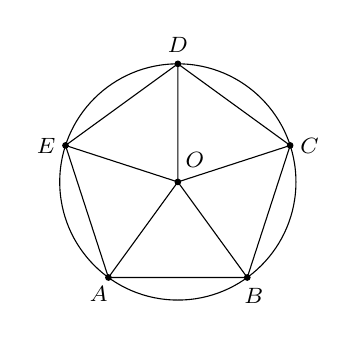
\begin{tikzpicture}[>=stealth,line join=round,line cap=round,font=\footnotesize,scale=1]
			%Hình ngũ giác đều
			\path 
			(0,0) coordinate (O)++(90:1.5) coordinate (D)
			(18:1.5) coordinate (C)
			(162:1.5) coordinate (E)
			(234:1.5) coordinate (A)
			(306:1.5) coordinate (B)
			;
			\draw (A)--(B)--(C)--(D)--(E)--cycle(A)--(O)--(B)(O)--(C)(O)--(D)(O)--(E)
			;
			\draw (O) circle (1.5);
			\foreach \t/\g in {A/-120,B/-70,C/0,D/90,E/180}{
				\draw[fill=black] (\t) circle (1pt) node[shift={(\g:7pt)}]{$\t$};}
			\draw[fill=black] (O) circle (1pt) node[shift={(52:3.5mm)}]{$O$};
	\end{tikzpicture}}
	\loigiai{
		\begin{enumerate}
			\item Vì $ABCDE$ là ngũ giác đều nội tiếp đường tròn $(O)$ nên $\wideparen{AB}=\wideparen{BC}= \wideparen{CD}=\wideparen{DE}=\wideparen{EA}$.\\
			Suy ra $\text{sđ} \wideparen{AB}=\text{sđ} \wideparen{BC}= \text{sđ} \wideparen{CD}=\text{sđ} \wideparen{DE}=\text{sđ} \wideparen{EA}=\dfrac{360^\circ}{5}=72^\circ$.
			\item $5$ phép quay giữ nguyên ngũ giác đều $ABCDE$ là các phép quay thuận chiều tâm $O$ với các góc quay lần lượt là $72^\circ$, $144^\circ$, $216^\circ$, $288^\circ$, $360^\circ$.
		\end{enumerate}
	}
\end{bt}

\begin{bt}%[SGK CTST Toán 9]%[Dự án EX-9-Đề Cương Toán 9]%[Nguyễn Tiến Liên]%[9H3H3-2]
	Tìm phép quay biến hình ngũ giác đều tâm $I$ thành chính nó.
	\begin{center}
		\begin{tikzpicture}[>=stealth,line join=round,line cap=round,font=\footnotesize,scale=1]
			\def\r{1.6}
			\path (0:0) coordinate (I) 
			(90:\r) coordinate (M)
			(18:\r) coordinate (N)
			(-54:\r) coordinate (P)
			(-126:\r) coordinate (Q)
			(162:\r) coordinate (R);
			\draw[fill=yellow!10]
			(M)--(N)--(P)--(Q)--(R)--cycle
			;
			\draw[red] 
			(I)--(M)
			(I)--(N)
			(I)--(P)
			(I)--(Q)
			(I)--(R)
			;
			\foreach \x/\g in {M/90,N/30,P/-45,Q/-135,R/150,I/-90}
			\fill[black] 	(\x) circle(1pt)
			($(\g:3mm)+(\x)$) node {$\x$};
		\end{tikzpicture}
	\end{center}	
	\loigiai{
		\immini{
			Năm đỉnh $M$, $N$, $P$, $Q$, $R$ của ngũ giác đều $MNPQR$ chia đường tròn $(O)$ thành năm cung bằng nhau, mỗi cung có số đo $72^\circ$. Từ đó, các phép quay biến ngũ giác đều $MNPQR$ thành chính nó là các phép quay $72^\circ$, $144^\circ$, $216^\circ$, $288^\circ$ hoặc $360^\circ$ tâm $I$ cùng chiều kim đồng hồ hoặc ngược chiều kim đồng hồ.		
		}
		{
			\begin{tikzpicture}[>=stealth,line join=round,line cap=round,font=\footnotesize,scale=1]
				\def\r{1.6}
				\path (0:0) coordinate (I) 
				(90:\r) coordinate (M)
				(18:\r) coordinate (N)
				(-54:\r) coordinate (P)
				(-126:\r) coordinate (Q)
				(162:\r) coordinate (R);
				\draw[fill=yellow!10]
				(M)--(N)--(P)--(Q)--(R)--cycle
				;
				\draw (I) circle (\r);
				\draw[red] 
				(I)--(M)
				(I)--(N)
				(I)--(P)
				(I)--(Q)
				(I)--(R)
				;
				\foreach \x/\g in {M/90,N/30,P/-45,Q/-135,R/150,I/-90}
				\fill[black] 	(\x) circle(1pt)
				($(\g:3mm)+(\x)$) node {$\x$};
			\end{tikzpicture}
		}
	}
\end{bt}

\begin{bt}%[Dự án EX-9-Đề Cương Toán 9]%[Nguyễn Tiến Liên]%[9H3H3-2]
	\immini{Cho hình vuông $ABCD$, $O$ là giao điểm của hai đường chéo như hình bên. Hãy chỉ ra một phép quay biến hình vuông $ABCD$ thành chính nó.}{
		\begin{tikzpicture}[>=stealth,line join=round,line cap=round,font=\footnotesize,scale=1]
			%Hình vuông
			\path (0,0) coordinate (O)++(45:2) coordinate (B)	
			(135:2) coordinate (A)
			(-135:2) coordinate (D)
			(-45:2) coordinate (C);
			\draw (A)--(B)--(C)--(D)--cycle (A)--(C)(B)--(D);
			\foreach \x/\y/\z in {D/A/B,A/B/C,B/C/D,C/D/A,B/O/A}{
				\draw pic[draw, angle radius=2mm]{right angle = \x--\y--\z};}
			\foreach \t/\g in {O/-90,A/90,B/90,C/-90,D/-90}{
				\draw[fill=black] (\t) circle (1pt) node[shift={(\g:7pt)}]{$\t$};}
	\end{tikzpicture}}
	\loigiai{
		Xét hình vuông $ABCD$ có $OA=OB=OC=OD$ (tính chất hình vuông) nên $B$, $C$, $D$ thuộc đường tròn $(O;OA)$ và $\widehat{AOB}= \widehat{BOC}=\widehat{COD}=\widehat{DOA}=90^\circ$.\\
		Sử dụng phép quay thuận chiều $90^\circ$ tâm $O$: biến $A$ thành $B$, biến $B$ thành $C$, biến $C$ thành $D$, biến $D$ thành $A$.\\
		Suy ra phép quay trên biến hình vuông $ABCD$ thành chính nó.  
	}
\end{bt}

\begin{bt}%[Dự án EX-9-Đề Cương Toán 9]%[Nguyễn Tiến Liên]%[9H3N3-2]
	\immini{Cho tam giác đều $ABC$ nội tiếp đường tròn $(O)$. Hãy chỉ ra phép quay biến điểm $A$ thành điểm $B$, điểm $B$ thành điểm $C$ và điểm $C$ thành điểm $A$.}{
		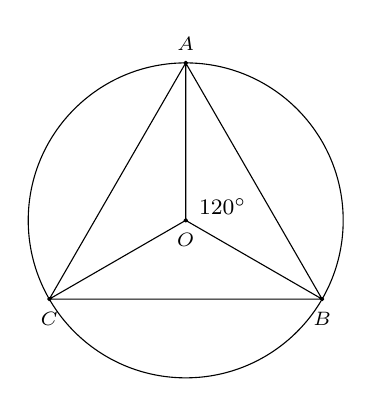
\begin{tikzpicture}[>=stealth,line join=round,line cap=round,font=\footnotesize,scale=1]	
		%Hình tam giác đều
		\path (0,0) coordinate (O)++(90:2) coordinate (A)	
		(-30:2) coordinate (B)
		(-150:2) coordinate (C);
		\draw (A)--(C)--(B)--(A) (O)--(A)(O)--(B)(O)--(C);
		\draw (O) circle (2);
		\draw (20:.5)node{$120^\circ$};
		\foreach \t/\g in {A/90,B/-90,C/-90,O/-90}{
		\draw[fill=black] (\t) circle (.6pt) node[shift={(\g:7pt)},font=\scriptsize]{$ \t $};}
		\end{tikzpicture}
}
	\loigiai{
	Phép quay thuận chiều $120^\circ$ tâm $O$ hoặc phép quay ngược chiều $240^\circ$ tâm $O$ biến điểm $A$ thành điểm $B$, điểm $B$ thành điểm $C$ và điểm $C$ thành điểm $A$.
	}
\end{bt}

\begin{bt}%[Dự án EX-9-Đề Cương Toán 9]%[Nguyễn Tiến Liên]%[9H3H3-2]
	\immini{Cho hình ngôi sao $6$ cánh (Hình bên) có các đỉnh $A$, $B$, $C$, $D$, $E$, $F$ nằm trên $(O)$ và đa giác $ABCDEF$ là lục giác đều.
		\begin{enumerate}
			\item Có bao nhiêu phép quay thuận chiều $\alpha^\circ$ ($0^\circ < \alpha \leq 360^\circ$) tâm $O$ biến ngôi sao (hình bên) thành chính nó?
			\item Với phép quay $\alpha = 120^\circ$ và $\alpha = 240^\circ$ tâm $O$, ngược chiều kim đồng hồ biến điểm $A$ thành điểm nào?
		\end{enumerate}
	}{
		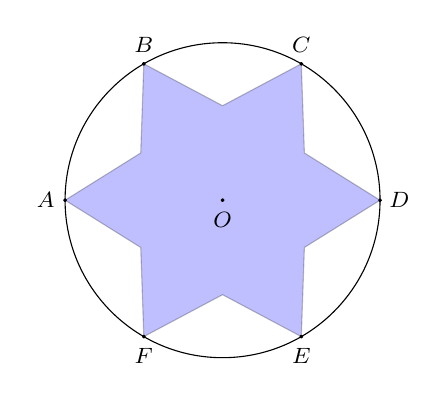
\begin{tikzpicture}[>=stealth,line join=round,line cap=round,font=\footnotesize,scale=1]
			%Hình lục giác đều
			\path (0,0) coordinate (O)++(0:2) coordinate (D)	
			(60:2) coordinate (C)
			(120:2) coordinate (B)
			(180:2) coordinate (A)
			(240:2) coordinate (F)
			(300:2) coordinate (E)
			(90:1.2) coordinate (A1)	
			(30:1.2) coordinate (A6)
			(150:1.2) coordinate (A2)
			(210:1.2) coordinate (A3)
			(270:1.2) coordinate (A4)
			(330:1.2) coordinate (A5);
			\draw[fill=blue,opacity=.25] (C)--(A1)--(B)--(A2)--(A)--(A3)--(F)--(A4)--(E)--(A5)--(D)--(A6)--cycle
			;
			\draw (O) circle (2);
			\foreach \t/\g in {O/-90,A/180,B/90,C/90,D/0,E/-90,F/-90}{
				\draw[fill=black] (\t) circle (.5pt) node[shift={(\g:7pt)}]{$\t$};}
	\end{tikzpicture}}
	\loigiai{
		\begin{enumerate}
			\item Có $6$ phép quay thuận chiều thỏa mãn yêu cầu bài toán, là các phép quay  $60^\circ$; $120^\circ$; $180^\circ$; $240^\circ$;$300^\circ$; $360^\circ$ tâm $O$ biến ngôi sao thành chính nó.
			\item Với phép quay ngược chiều $\alpha = 120^\circ$ tâm $O$ biến điểm $A$ thành điểm $E$, phép quay ngược chiều $\alpha = 240^\circ$ biến điểm $A$ thành điểm $C$.
		\end{enumerate}
	}
\end{bt}

\begin{bt}%[Dự án EX-9-Đề Cương Toán 9]%[Nguyễn Tiến Liên]%[9H3H3-2]
	Một phép quay thuận chiều $120^\circ$ tâm $O$ biến điểm $A$ thành điểm $B$, biến điểm $B$ thành điểm $C$. Chứng tỏ rằng $ABC$ là tam giác đều nội tiếp một đường tròn tâm $O$.
	\loigiai{ 
		\begin{center}
			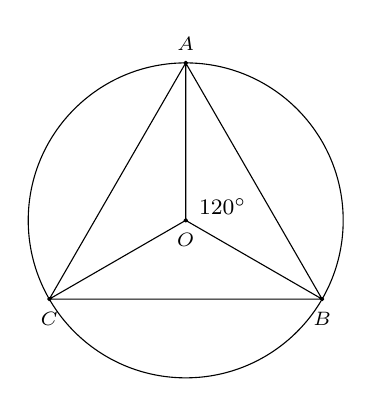
\begin{tikzpicture}[>=stealth,line join=round,line cap=round,font=\footnotesize,scale=1]	
				%Hình tam giác đều
				\path (0,0) coordinate (O)++(90:2) coordinate (A)	
				(-30:2) coordinate (B)
				(-150:2) coordinate (C);
				\draw (A)--(C)--(B)--(A) (O)--(A)(O)--(B)(O)--(C);
				\draw (O) circle (2);
				\draw (20:.5)node{$120^\circ$};
				\foreach \t/\g in {A/90,B/-90,C/-90,O/-90}{
					\draw[fill=black] (\t) circle (.6pt) node[shift={(\g:7pt)},font=\scriptsize]{$ \t $};}
			\end{tikzpicture}
		\end{center}
		Ta có $OA = OB = OC$.\\
		Vậy tam giác $ABC$ nội tiếp đường tròn $(O)$.\\
		Hơn nữa các cung nhỏ $\wideparen{AB}$, $\wideparen{BC}$ có số đo bằng $120^\circ$.\\
		Vì $\widehat{ACB}$ và $\widehat{BAC}$ là các góc nội tiếp của $(O)$ lần lượt chắn cung $\wideparen{AB}$, $\wideparen{BC}$ nên
		$\widehat{ACB} = \dfrac{1}{2} \text{sđ}\wideparen{AB} = 60^\circ$ và $\widehat{BAC} = \dfrac{1}{2} \text{sđ}\wideparen{BC} = 60^\circ$.\\
		Suy ra $\widehat{ABC} = 180^\circ - \widehat{ACB} - \widehat{BAC} = 60^\circ$.\\
		Do đó tam giác $ABC$ có ba góc bằng nhau.\\
		Vậy tam giác $ABC$ là tam giác đều.
	}
\end{bt}

\begin{bt}%[Dự án EX-9-Đề Cương Toán 9]%[Nguyễn Tiến Liên]%[9H3V3-2]
Cho hình vuông $ABCD$ nội tiếp đường tròn $(O)$. Phép quay thuận chiều $45^\circ$ tâm $O$ biến điểm $A$ thành điểm $E$, điểm $B$ thành điểm $F$, điểm $C$ thành điểm $G$, điểm $D$ thành điểm $H$.
\begin{enumerate}
	\item Chứng minh rằng $AEBFCGDH$ là hình bát giác đều.
	\item Ta cần thực hiện hiện phép quay thuận chiều $\alpha^\circ$ tâm $O$ bằng bao nhiêu để điểm $B$ biến thành điểm $A$?
\end{enumerate}
	\loigiai{
			\begin{center}
			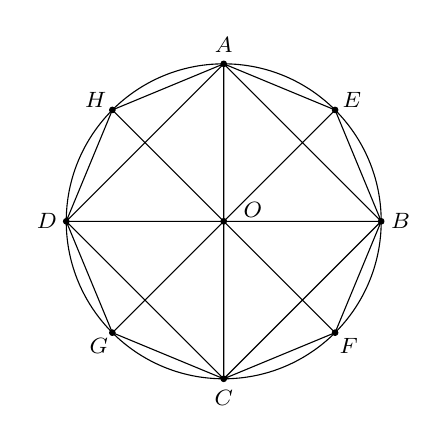
\begin{tikzpicture}[>=stealth,line join=round,line cap=round,font=\footnotesize,scale=1]	
				\path (0,0) coordinate (O)++(90:2) coordinate (A)	
				(0:2) coordinate (B)
				(-90:2) coordinate (C)
				(180:2) coordinate (D)
					(45:2) coordinate (E)
				(135:2) coordinate (H)
				(225:2) coordinate (G)
				(315:2) coordinate (F);
				\draw (O) circle (2);
				\draw (A)--(B)--(C)--(D)--cycle (E)--(G)(H)--(F)(A)--(C)(B)--(D)(A)--(E)--(B)--(F)--(C)--(G)--(D)--(H)--cycle
				;	
				\foreach \t/\g in {A/90,B/0,C/-90,D/180,E/30,H/150,G/-135,F/-45}{
					\draw[fill=black] (\t) circle (1pt) node[shift={(\g:7pt)}]{$ \t $};}
				\draw[fill=black] (O) circle (1pt) node[shift={(22:4mm)}]{$O$};
			\end{tikzpicture}
		\end{center}
		\begin{enumerate}
		\item 
		Ta có $\text{sđ}\wideparen{AE} = \text{sđ}\wideparen{EB} = \text{sđ}\wideparen{BF} = \text{sđ}\wideparen{FC}=\text{sđ} \wideparen{CG}=\text{sđ} \wideparen{GD}=\text{sđ} \wideparen{DH}=\text{sđ} \wideparen{HA}=\dfrac{360^\circ}{8}=45^\circ$.\\
		Suy ra $\widehat{AOE}= \widehat{EOB}=\widehat{BOF}=\widehat{FOC}=\widehat{COG}= \widehat{GOD}=\widehat{DOH}=\widehat{HOA}=45^\circ$ (các góc ở tâm chắn các cung bằng nhau).\\
		Suy ra $\triangle{AOE}= \triangle{EOB}=\triangle{BOF}=\triangle{FOC}=\triangle{COG}= \triangle{GOD}=\triangle{DOH}=\triangle{HOA}$.\\
		Do đó
		\begin{itemize}
			\item $AE=EB=BF=FC=CG=GD=DH=HA$.
			\item $\widehat{HAE}= \widehat{AEB}=\widehat{EBF}=\widehat{BFC}=\widehat{FCG}= \widehat{CGD}=\widehat{GDH}=\widehat{DHA}=135^\circ$.
		\end{itemize}
		Vậy $AEBFCGDH$ là hình bát giác đều.
		\item Để điểm $B$ biến thành điểm $A$, ta cần thực hiện phép quay thuận chiều $270^\circ$ tâm $O$.
		\end{enumerate}
	}
\end{bt}

\begin{bt}%[Dự án EX-9-Đề Cương Toán 9]%[Nguyễn Tiến Liên]%[9H3H3-3]
	\immini{Đường viền đồng hồ treo tường (Hình bên) là một đa giác đều.
		\begin{enumerate}
			\item Đồng hồ được làm theo hình đa giác đều nào? Tính số đo mỗi góc của đa giác đó.
			\item Tìm các phép quay quay thuận chiều $\alpha^\circ$ ($0^\circ < \alpha \leq 360^\circ$) biến đa giác này thành chính nó.
		\end{enumerate}
	}{
\begin{tikzpicture}[>=stealth,line cap=round,line join=round,line width=3pt,font=\footnotesize,scale=0.9]
	\def \h{49} %vị trí kim giờ
	\def \m{60} %vị trí kim phút
	\def \s{30} %vị trí kim giây
	\path
	(0,0) coordinate (O);
	\fill [fill=yellow!20] (0,0) circle (2.2cm);
	\foreach \angle / \label in
	{0/3, 30/2, 60/1, 90/12, 120/11, 150/10, 180/9,
		210/8, 240/7, 270/6, 300/5, 330/4}
	{
		\draw[line width=1pt] (\angle:1.8cm) -- (\angle:2cm);
		\draw (\angle:1.4cm) node{\textsf{\label}};
	}
	\foreach \angle in {0,90,180,270}
	\draw[line width=2pt] (\angle:1.6cm) -- (\angle:2cm);
	%\node[draw=none,font=\tiny,text=red] at (0,-0.7cm) {THĂNG LONG};
	\draw[rotate=90,line width=2pt] (0,0) -- (-\h*6-\m*30/60:0.7cm); % hours
	\draw[rotate=90,line width=1.5pt] (0,0) -- (-\m*6:1cm); % minutes
	%\draw[rotate=90,thin,red] (0,0) -- (-s*6:1.2cm); % seconds
	%\path [fill=red] (0,0) circle (2pt);
	\draw[line width=0.3cm,color=brown!60] ($(O) + (22.5:2.2)$)--($(O) + (67.5:2.2)$)--($(O) + (112.5:2.2)$)--($(O) + (157.5:2.2)$)--($(O) + (202.5:2.2)$)--($(O) + (247.5:2.2)$)--($(O) + (292.5:2.2)$)--($(O) + (337.5:2.2)$)--cycle;
	\end{tikzpicture}}
	\loigiai{
		\begin{enumerate}
			\item Đồng hồ được làm theo hình bát giác đều.
			Số đo mỗi góc của đa giác đều $n$ cạnh được tính bằng công thức $\dfrac{(n-2)\cdot 180^\circ}{n}$.\\
			Do đó số đo mỗi góc của hình bát giác đều là $\dfrac{(8-2)\cdot 180^\circ}{8}=135^\circ$.
			\item Gọi $O$ là tâm hình bát giác đều ở trên.\\
			 Có $8$ phép quay thuận chiều thuận chiều $\alpha^\circ$ ($0^\circ < \alpha \leq 360^\circ$) thỏa mãn yêu cầu bài toán, là các phép quay $45^\circ; 90^\circ; 135^\circ; 180^\circ; 225^\circ; 270^\circ; 315^\circ; 360^\circ$ tâm $O$ biến hình bát giác đều này thành chính nó.
		\end{enumerate}
	}
\end{bt}

\begin{bt}%[Dự án EX-9-Đề Cương Toán 9]%[Nguyễn Tiến Liên]%[9H3H3-2]
	\immini{Một vòng quay may mắn có dạng là một hình đa giác đều $10$ cạnh (Hình bên). Tìm các phép quay ngược chiều $\alpha^\circ$ ($0^\circ < \alpha \leq 360^\circ$) biến đa giác này thành chính nó.}
	{	%%%%%%%%%%%Hình vòng quay X-Đ-T-V các màu
		\begin{tikzpicture}[line join = round, line cap=round,>=stealth,font=\footnotesize,scale=0.4]
			%			\draw (0,0) circle (5cm);
			\draw[fill=black] (0,0)--(-110:6)--(-70:6)--cycle;
			\foreach \x in {90,126,162,198,234,270,306,342,378,414}{
				\coordinate (A\x) at (\x:5);
				\draw (0,0)--(\x:5)
				;
			}
			\fill[red] (A90) --(A126)--(0,0)--cycle; 
			\fill[yellow] (A126) --(A162)--(0,0)--cycle; 
			\fill[pink] (A162) --(A198)--(0,0)--cycle; 
			\fill[brown] (A198) --(A234)--(0,0)--cycle ; 
			\fill[green] (A198) --(A234)--(0,0)--cycle; 
			\fill[violet] (A234) --(A270)--(0,0)--cycle; 
			\fill[magenta] (A270) --(A306)--(0,0)--cycle; 
			\fill[orange] (A306) --(A342)--(0,0)--cycle; 
			\fill[green!50!black] (A342) --(A378)--(0,0)--cycle; 
			\fill[blue] (A378) --(A414)--(0,0)--cycle; 
			\draw (A90)--(A414);
			
			\draw[fill=yellow!50!black] (0,0) circle (1cm);
			
			\draw[fill=black] (0,0) circle (0.6cm);
			\draw[fill=white] (0,0) circle (0.5cm);
			\draw[fill=black] 
			(120:0.6) -- (95:2)--($(95:2)+(-0.3,0)$)--(90:2.5)--($(85:2)+(0.3,0)$)--(85:2)--(60:0.6)
			;
		\end{tikzpicture}
	}
	\loigiai{
		Gọi $(O)$ là đường tròn ngoại tiếp hình đa giác đều $10$ cạnh ở trên.\\
		$10$ đỉnh của đa giác đều chia đường tròn thành $10$ cung bằng nhau, mỗi cung có số đo $\dfrac{360^\circ}{10}=36^\circ$.\\
		Vậy có $10$ phép quay ngược chiều $\alpha^\circ$ ($0^\circ < \alpha \leq 360^\circ$) thỏa mãn yêu cầu bài toán, là các phép quay $36^\circ$; $72^\circ$; $108^\circ$; $144^\circ$; $180^\circ$; $216^\circ$; $252^\circ$; $288^\circ$; $324^\circ$; $360^\circ$ tâm $O$ biến vòng quay may mắn thành chính nó.
	}
\end{bt}

%===========/ Bài tập trắc nghiệm/===========
\subsection{Bài tập trắc nghiệm}
\Opensolutionfile{ans}[ans/ans-9C9-B3]
\setcounter{ex}{0}
%Câu1
\begin{ex}%[Dự án EX-9-Đề Cương Toán 9]%[Nguyễn Tiến Liên]%[9H3N3-1]
	Cho đa giác đều $\mathcal{H}$ có ${72}$ cạnh, nội tiếp một đường tròn $(O)$. Kẻ các đoạn thẳng nối $O$ với các đỉnh của $\mathcal{H}$ và thu được $72$ góc nhọn tại đỉnh $O$ (không chồng lên nhau). Số đo của các góc nhọn này bằng bao nhiêu?
	\choice
	{\True $5^\circ$}
	{$13^\circ$}
	{$2^\circ$}
	{$7^\circ$}
	\loigiai{ 
		Số đo của góc nhọn tại đỉnh $O$ là $360^\circ \div 72 ^\circ$.
	}
\end{ex}
%Câu2
\begin{ex}%[Dự án EX-9-Đề Cương Toán 9]%[Nguyễn Tiến Liên]%[9H3N3-2]
	Cho đa giác đều $\mathcal{H}$ có $30$ cạnh, nội tiếp một đường tròn $(O)$. Kẻ các đoạn thẳng nối $O$ với các đỉnh của $\mathcal{H}$ và thu được $30$ góc nhọn tại đỉnh $O$ (không chồng lên nhau). Phép quay nào sau đây không giữ nguyên hình?
	\choice
	{Phép quay ngược chiều tâm $O$ với góc quay $36^\circ$}
	{Phép quay thuận chiều tâm $O$ với góc quay $12^\circ$}
	{\True Phép quay thuận chiều tâm $O$ với góc quay $13^\circ$}
	{Phép quay ngược chiều tâm $O$ với góc quay $24^\circ$}
	\loigiai{ 
		Số đo của góc nhọn tại đỉnh $O$ là $360^\circ \div 30=12 ^\circ$, nên phép quay giữ nguyên hình là phép quay tâm $O$ góc quay $k\cdot 12 ^\circ$ với $k$ là số tự nhiên.
	}
\end{ex}
%Câu3
\begin{ex}%[Dự án EX-9-Đề Cương Toán 9]%[Nguyễn Tiến Liên]%[9H3N3-2]
	Cho tam giác đều $BFK$ nội tiếp đường tròn tâm $O$, phép quay ngược chiều tâm O góc quay $360^\circ$ biến điểm $B$ thành điểm nào?  
	\choice
	{\True $B$}
	{$F$}
	{$O$}
	{$K$}
	\loigiai{ 
		Phép quay ngược chiều tâm $O$ góc quay $360^\circ$ biến điểm $B$ thành điểm $B$.
	}
\end{ex}
%Câu4
\begin{ex}%[Dự án EX-9-Đề Cương Toán 9]%[Nguyễn Tiến Liên]%[9H3N3-2]
	Cho hình vuông $ACJM$ nội tiếp đường tròn tâm $O$, phép quay ngược chiều tâm $O$ góc quay $180^\circ$ biến điểm $A$ thành điểm nào? 
	\choice
	{$M$}
	{$A$}
	{\True $J$}
	{$C$}
	\loigiai{ 
	Phép quay ngược chiều tâm O góc quay $180^\circ$ biến điểm $A$ thành điểm $J$.}
\end{ex}
%Câu5
\begin{ex}%[Dự án EX-9-Đề Cương Toán 9]%[Nguyễn Tiến Liên]%[9H3N3-2]
	Cho ngũ giác đều $CFKLN$ nội tiếp đường tròn tâm $O$, phép quay ngược chiều tâm O góc quay $144^\circ$ biến điểm $C$ thành điểm nào? 
	\choice
	{$N$}
	{\True $L$}
	{$K$}
	{$F$}
	\loigiai{ 
		Phép quay ngược chiều tâm $O$ góc quay $144^\circ$ biến điểm $C$ thành điểm $L$.
	}
\end{ex}

% In đáp án trắc nghiệm
\Closesolutionfile{ans}
\indapan{6}{ans/ans-9C9-B3}


